% concatenated from main.tex, preamble.tex, main/introduction.tex, main/overview.tex, main/r_neighborhood_exact_relaxations.tex, main/averaging_lemma.tex, main/sampling_distributions.tex, main/proof_main_theorem_1.tex, main/hypergraph_matching.tex, main/extended_formulations_small_rhs.tex, main/appendix.tex
\documentclass[11pt]{article}

\usepackage[letterpaper,margin=1in]{geometry}
\usepackage{setspace}

% Single spacing between lines
\singlespacing
 
% Extra space between paragraphs
\setlength{\parskip}{0.8em}

%=======================================================
% usepackage
\usepackage[T1]{fontenc}
\usepackage{baskervillef}
\usepackage[varqu,varl,var0]{inconsolata}
\usepackage[scale=.95,type1]{cabin}
\usepackage[baskerville,vvarbb]{newtxmath}
\usepackage[cal=boondoxo]{mathalfa}
\usepackage{latexsym}
\let\Bbbk= \undefined
\usepackage{amssymb}
\let\openbox = \undefined
\usepackage{geometry}
\geometry{a4paper}
\usepackage{graphicx}
\usepackage{epstopdf}
\usepackage{enumerate}
\usepackage{xcolor}
\usepackage{amsthm}
\usepackage{amscd}
\usepackage{amsmath}
\usepackage{thm-restate}
\usepackage{subfiles}
\usepackage{hyperref}
\usepackage{tikz}
\usepackage{subcaption}
\usepackage{utf8math}

\usepackage{todonotes}


% \usepackage[backend=biber, maxbibnames=99, sorting=nyt, style=ieee, giveninits=true]{biblatex}
% \addbibresource{papers.bib}
% \addbibresource{mybib.bib}
% \addbibresource{books.bib}
% \addbibresource{refs.bib}


% % Disable some fields for references (mainly from refs.bib)
% \ExecuteBibliographyOptions{
%     doi=false,
%     isbn=false,
%     url=false,
%     eprint=false
% }


% Define a custom color named 'cyantransparent' with 50% opacity
\colorlet{cyantransparent}{cyan!50} 
\colorlet{pinktransparent}{pink!50} 
\colorlet{greentransparent}{green!45}


\newcommand{\fritztodo}[1]{\todo[backgroundcolor=cyantransparent, linecolor=cyan!80]{#1}}
\newcommand{\larstodo}[1]{\todo[backgroundcolor=pinktransparent, linecolor=pink!80]{#1}}
\usetikzlibrary{arrows.meta,decorations.markings}
\newcommand{\jiayetodo}[1]{\todo[backgroundcolor=greentransparent, linecolor=green!80]{#1}}
\usetikzlibrary{arrows.meta,decorations.markings}


\DeclareMathOperator{\support}{support}

\newcommand{\R}{\mathbb{R}}
\newcommand{\NP}{{\sf NP}}
\newcommand{\Z}{\mathbb{Z}}
\newcommand{\one}{\mathbf{1}}
\newcommand{\zero}{\mathbf{0}}

% Jiaye: I changed these two new commands by adding \left and \right.
\newcommand{\floor}[1]{\left\lfloor #1 \right\rfloor}
\newcommand{\ceil}[1]{\left\lceil #1 \right\rceil}

%\newcommand{\Pr}{\mathop{\rm Pr}}

\DeclareMathOperator{\ones}{ones}
\DeclareMathOperator{\supp}{supp}
\DeclareMathOperator{\conv}{conv}
\DeclareMathOperator{\forcing}{forcing}
\DeclareMathOperator{\forcingset}{forcing-set}

% \newcommand{\proba}{\mathbb{P}}
\newcommand{\proba}{\Pr}

%Parameters
\newcommand{\eps}{\varepsilon} 
\newcommand{\numrounds}{t}
\newcommand{\rhs}{\delta}
\newcommand{\covproba}{\gamma}
\newcommand{\numrows}{r}
\newcommand{\threshold}{\tau}

\newtheorem{theorem}{Theorem}
\newtheorem{lemma}[theorem]{Lemma}
\newtheorem{proposition}[theorem]{Proposition}


%\newcommand{\todo{{\color{red}TODO. }}

\DeclareGraphicsRule{.tif}{png}{.png}{`convert #1 `dirname #1`/`basename #1 .tif`.png}

\newcommand{\sam}[1]{{\color{magenta}Sam: {#1} }}
\newcommand{\lars}[1]{{\color{magenta}Lars: {#1} }}
\newcommand{\fritz}[1]{{\color{magenta}Fritz: {#1} }}
\newcommand{\jiaye}[1]{{\color{magenta}Jiaye: {#1} }}

% Jiaye's shortcuts
\newcommand{\rb}[1]{\left(#1\right)}
\newcommand{\set}[1]{\left\{#1\right\}}
\newcommand{\norm}[1]{\left\lVert#1\right\rVert}
\newcommand{\opt}{\text{OPT}}
\renewcommand{\epsilon}{\varepsilon}

\theoremstyle{remark}
\newtheorem{remark}{Remark}

% \newcommand{\todo}[1]{{\color{magenta}TODO: {#1} }}

% Lars: I think we should stick to standard typesetting including indents
%\setlength{\parindent}{0pt}

%%% Local Variables:
%%% mode: LaTeX
%%% TeX-master: "../main"
%%% End:


\usepackage[
    style=numeric, % Or 'numeric', 'ieee', etc.
    natbib=true,      % Allows you to keep using \citep and \citet
    doi=false,        % This solves your DOI problem
    url=false,        % This solves your URL problem
    isbn=false,       % Optional: removes ISBN
%    giveninits=true, 
    backend=biber,     % Recommended backend
    maxbibnames=99,
    minbibnames=99
]{biblatex}

%\usepackage[backend=biber, style=numeric, giveninits=true,maxbibnames=99,
 % minbibnames=99]{biblatex}
\addbibresource{papers.bib}
\addbibresource{mybib.bib}
\addbibresource{books.bib}
\addbibresource{refs.bib}



\title{Polyhedral extended formulations that approximate the Gomory closure for packing problems} 
\author{
Friedrich Eisenbrand \thanks{EPFL, Lausanne, Switzerland, \texttt{\{friedrich.eisenbrand, jiaye.wei\}@epfl.ch}}
\and
Samuel Fiorini \thanks{Université libre de Bruxelles, Brussels, Belgium, \texttt{Samuel.Fiorini@ulb.be}}
\and
Lars Rohwedder \thanks{University of Southern Denmark, Odense, Denmark, \texttt{rohwedder@sdu.dk}}
\and
Jiaye Wei \footnotemark[1]
}
\date{} % no date
\begin{document}
\maketitle

\begin{abstract}
  \noindent
  We consider $0/1$ packing problems  $\max\{c^\intercal x ： Ax≤\one, \, x ∈ \{0,1\}^n\}$, with $A ∈ ℝ_{≥0}^{m ×n}$. A way to solve such problems is via tightening  the linear programming relaxation  $P$ % = \{x ∈ [0,1]^n ： Ax≤\one\}$
  with Gomory  \emph{cutting-planes}.  The Gomory-closure $P'$ of $P$ is the intersection of $P$ with all its cutting planes. 
  The optimization problem over $P'$  is \NP-hard. Mastrolilli (2020) has shown that for fixed $ε>0$, the  Lasserre hierarchy yields a  polynomial-size convex but non-polyhedral extended formulation that approximates $P'$ up to a factor of $1+ε$.  Our main result is the construction of a polyhedral and polynomial extended formulation that approximates $P'$ with the same approximation guarantee. Our construction is based on first principles. Like Mastrolilli's approach, ours also applies to higher iterates $P^{(t)}$ for fixed $t$ and $ε>0$.  

  In contrast to an explicit construction, communication complexity
  provides an alternative way to describe extended formulations. Using
  this approach we obtain a quasi-polynomial polyhedral extended
  formulation for the  above problem that is superior in some parameter regimes. To
  achieve this, we describe a communication protocol extending
  Yannakakis'  protocol to decide whether the clique of Alice
  and the stable set of Bob intersect.
  
  
\end{abstract}


\section{Introduction}
\label{sec:introduction}
% \larstodo{@Jiaye: use $\Z_{\ge 1}$ / $\Z_{\ge 0}$ instead of $\mathbb N$ / $\mathbb N_1$ everywhere}


An \emph{integer program} is a problem of the form
\begin{equation}
  \label{eq:01-ip}
  \max \{c^\intercal x ： x ∈ ℤ^n, Ax ≤ b \},  
\end{equation}
with $c ∈ ℤ^n$, $A ∈ ℤ^{m ×n}$ and $b ∈ ℤ^m$. This framework captures many important \NP-hard optimization problems, see, e.g~\cite{Schrijver03,wolsey2020integer}. Successful approaches to tackle~(\ref{eq:01-ip}) are largely based on the solution of the \emph{linear relaxation} %of~(\ref{eq:01-ip})
%\begin{equation}
%  \label{eq:01-ip}
  $\max \{c^\intercal x ： x ∈ ℝ^n, Ax ≤ b \}$. % \footnote{We assume that the variable upper bound $x≤ \one$ is implicit in $Ax≤b$} 
%\end{equation}
%of~(\ref{eq:01-ip}) instead.
  The linear relaxation can be solved efficiently and it provides upper bounds, also for sub-problems of~(\ref{eq:01-ip}) that then help in pruning the search space. 
  The efficiency of this approach depends on the quality of the linear relaxation.

  \emph{Cutting planes} provide a way to strengthen the linear relaxation.  The principle was invented by Gomory~\cite{Gomory58} who made the following important observation.  %\fritztodo{Gomory is more general}
Denote the polyhedron of feasible solutions of the linear relaxation by $P$.  If $c ∈ℤ^n$ is an integer vector and the inequality $c^\intercal x ≤ δ$ is satisfied by each $x ∈ P$ , then
\begin{equation}
  \label{eq:3}
  c^\intercal x ≤ ⌊δ ⌋
\end{equation}
is satisfied by each feasible \emph{integral}  $x ∈ P ∩ℤ^n$ in the relaxation. Based on this principle, Chvátal~\cite{Chvatal73} defined the notion of a \emph{closure operation} and  \emph{hierarchy}. % If $P ⊆ ℝ^n$ is a polyhedron, the feasible solutions of the relaxation in our case, then 
The \emph{first closure} $P'$  of $P$ is the intersection of all Gomory cutting planes that can be derived for $P$. If $P$ is a rational polyhedron, then $P'$  is a rational polyhedron again~\cite{MR597387}. Iterating this procedure $i$~times  yields a polyhedron denoted by $P^{(i)}$ and a finite, see~\cite{MR597387}, \emph{hierarchy}  $P ⊇ P' ⊇ P^{(2)} ⊇ \cdots ⊇ P^{(k)}=P_I$, where $P_I$ is the convex hull of all integral solutions, i.e. the \emph{integer hull} of $P$. The smallest number $k∈ \Z_{\geq 0}$, where $P^{(k)}$ equals $P_I$, is referred to as \emph{Chvátal rank} or simply \emph{rank} of $P$.

For relaxations $P ⊆[0,1]^n$ that are contained in the $0/1$-cube, other important hierarchies have been  developed since then, such as \emph{lift and project}~\cite{BCC96}, the hierarchies of Sherali and Adams~\cite{SheraliAdams90}, Lov{\'a}sz and Schrijver~\cite{LovaszSchrijver90} as well as the one of Lasserre~\cite{MR2041934}. The last two in this list are non-polyhedral relaxations that are based on \emph{semidefinite programming}. Common to all these specific hierarchies for the cube are two important features: a) Optimization over the $t$-th closure can be done in polynomial time for fixed $t$ and b) the corresponding rank of a polytope $P ⊆ [0,1]^n$ is bounded by $n$, see also~\cite{MR1997246}. 
% \subsection*{Main results}
This is not the case for the Gomory-closure of a polytope in the $0/1$-cube. The Chvátal rank of a polytope $P ⊆[0,1]^n$ is upper bounded by a polynomial in $n$~\cite{BEHS99,es03}, but there are cases, for which quadratic lower bounds hold~\cite{rothvoss20170}. Furthermore, optimizing over the first closure is \NP-hard~\cite{eisen99} even for polytopes in the $0/1$-cube~\cite{cornuejols2020rational,cornuejols2018gomory}.  On the other hand, the first Gomory-closure of the fractional matching polytope is already its integer hull~\cite{Edmonds65b}, while the rank of the fractional matching polytope has linear lower bounds w.r.t. the other hierarchies mentioned above~\cite{mathieu2009sherali,au2016comprehensive}. 


Bienstock and
Zuckerberg~\cite{bz06} provided a method to approximate the fixed-rank 
Gomory-closure of a \emph{covering problem} up to a scaling-factor of $1+ε$
 in
polynomial time. Recall that an integer program~\eqref{eq:01-ip} is a covering
problem, if the constraints are of the form $Ax≥\one, x ≥0$ for
$A ∈ ℝ^{m ×n}_{≥0}$. Fiorini et al.~\cite{fhw21} provided a simplified
approach with a complexity of $(mn)^{O(t/ε)}$ to approximate the
$t$th Gomory closure for $A ∈\{0,1\}^{m ×n}$. Their result is a \emph{linear (i.e., polyhedral) extended
  formulation } $E = \{(x,y) ∈ ℝ^{n+ℓ} ：Cx + Dy ≤ d \}$ such that the
\emph{projection} if this polyhedron $E$ to the $x$-variables yields a
corresponding relaxation. The stated complexity bound means that the number  $ℓ$ of additional variables, and
the number of constraints in the system $Cx+Dy≤d$ are bounded by
$(mn)^{O(t/ε)}$.%\larstodo{what about the coefficients?}


Gomory cutting planes are particularly strong for important \emph{packing problems} such as matching or hypergraph-matching problems~\cite{st10,cl12}. An integer program~\eqref{eq:01-ip} is a packing problem, if the constraints are of the form $Ax≤ \one, x≥0$ with $A ∈ ℝ_{≥0}^{m ×n}$. 
In this setting, Mastrolilli~\cite{mas20} provided a convex, but  non-linear extended formulation that approximates the fixed-rank Gomory-closure. His construction is based on the Lasserre / Sum-of-Squares (SoS) hierarchy. 


\subsubsection*{Contributions}

\emph{Our main result} is a linear-programming based extended formulation to approximate the fixed-rank Gomory-closure of packing problems.  
Linear programming is conceptionally much simpler than semidefinite programming and admits
highly scalable solvers in practice. 
The constructions that we use follow from first principles in linear programming such as the convex hull of a finite set of points, which typically exhibit good practical performance combined with standard approaches like
column generation and Dantzig-Wolfe decomposition, see e.g.~\cite{wolsey2020integer, dantzig1960decomposition}. 
A self-contained overview of the techniques for the first closure is in Section~\ref{sec:r-neighb-relax}.

% Main Theorem 1: Linear Approximation of CG Closure
\begin{restatable}{theorem}{approxcg}\label{thm:main-1}
    Let $P = \{x \in \R^n_{\ge 0} : Ax \le \one \}$ be a polytope contained in $[0,1]^n$, where $A \in \R_{\geq 0}^{m \times n}$. For each fixed $\eps \in (0,1/2)$ and $\numrounds\in \Z_{\geq 1}$, there exists a polyhedral relaxation $Q$ of the integer hull of $P$, which is a $(1+\eps)^\numrounds$-approximation of the $\numrounds$-th Gomory closure $P^{(t)}$ of $P$ and has a linear extended formulation of size
    \[
	    (nm)^{(1/\eps)^{O(\numrounds)}}\,.
    \]
%    \[
%    m^{(1/\eps)^\numrounds \mathrm{e}^{4\numrounds+O(1)} \ln(1+1/\eps)} n^{(1/\eps)^{2\numrounds} \mathrm{e}^{8\numrounds+O(1)} \ln(1+1/\eps)}.
%    \]
  \end{restatable}
  % 
% Approximation factors of the form $(1+\eps)^{\numrounds}$ are natural in our context, and help to keep the proofs as clean as possible. In case the reader wants an
  \begin{remark}
    To obtain a $(1+\tilde{\eps})$-approximation of $P^{(t)}$, one can simply replace $1/\eps$ by $t/\tilde{\eps}$ in the size bound of Theorem~\ref{thm:main-1}. See Appendix~\ref{appendix:approx-factor} for details. %\fritztodo{@Jiaye: Check please}\jiayetodo{Done! This is correct. I would suggest to have the computation of it in the appendix.}
  \end{remark}
  \begin{remark}
    We want to mention that a related, but much simpler approach, also succeeds for covering problems. The details are in  Appendix~\ref{appendix:covering}. 
  \end{remark}
\noindent 
The complexity of  the extended formulation in %size bound given in
Theorem~\ref{thm:main-1} is optimal for the first closure. %\larstodo{Could it be $(nm)^{t/\epsilon}$ like for covering?}
This follows from the exponential lower bound on the linear extension complexity of matching by Roth\-voss~\cite{rothvoss2017matching} and its generalization  for a $(1+\eps)$-approximation of the integer hull  by Sinha~\cite{sin18}. The author proved a $n^{\Omega(1/\eps)}$ lower bound on the size of any linear extended formulation providing a $(1+\eps)$-approximation of the integer hull of matchings. Recall that the first Gomory closure of the fractional matching polytope is integral. % and moreover $m = \Theta(\sqrt{n})$.\larstodo{is $\Theta$ really what we want to say or rather $\Omega(\cdot)$?. Could also be confusing because of typical use of $n=$ vertices, $m=$edges} 



\medskip
\noindent 
\emph{Matching problems} are a show-case for the strength of the Gomory closure. 
As mentioned above, the Gomory closure of the fractional matching polytope is the integral matching polytope. A generalization that has also received considerable attention in the recent literature is the \emph{unweighted} maximum matching problem in \emph{$k$-uniform hypergraphs}, also called \emph{$k$-set packing}.  A hypergraph $G = (V,E)$ is $k$-uniform, if each hyperedge consists of $k$ vertices. Chan and Lau~\cite{cl12} have shown that the integrality gap of  $Ω(n/k^3)$ rounds of the Sherali-Adams hierarchy on the standard LP relaxation remains at least $k− 2$. There are known polynomial time approximation algorithms that achieve a factor of $(k+1)/3$\cite{hurkens1989size,cygan2013improved,furer2014approximating}. Recently, Lee et al.~\cite{lee2025asymptotically} provided an inapproximability that matches this upper bound up to a constant. 

\smallskip 
\noindent
Singh and Talwar~\cite{st10} have shown that $O(k^2)$ iterations of the Gomory-closure operation suffice to reduce the integrality gap of the standard linear programming formulation to $(k+1)/2$.  We substantially improve this result. 
 \begin{restatable}{theorem}{hyper}\label{thm:hyper}
    For the maximum matching problem in $k$-uniform hypergraphs $G=(V,E)$, it suffices to apply $O(\log k)$ iterations of the Gomory-closure operation to the standard LP relaxation to reduce the integrality gap to $(k+1)/2$.
  \end{restatable}
% \larstodo{"rounds" is a bit inconsistent with our phrasing elsewhere.}
On a technical level, Theorem~\ref{thm:hyper} complements Theorem~\ref{thm:main-1}:
the proof of Theorem~\ref{thm:main-1} relies on enforcing additional local constraints in the relaxation,
which imply approximate Gomory cuts,
whereas the proof of Theorem~\ref{thm:hyper} uses that Gomory cuts imply similar local constraints that then lead
to a small integrality gap.


\medskip
\noindent 
\emph{Communication complexity} and communication protocols in particular provide a way to prove existence of extended formulations.
 Yannakakis'~\cite{Yannakakis91} protocol to determine whether the \emph{clique} of player \emph{Alice} and the \emph{stable set} of player \emph{Bob} intersect can be used to construct an extended formulation of the clique relaxation for stable set, see also~\cite{rao2020communication}. In general, the size of the formulation is singly exponential in the complexity of the protocol. For example, 
If the underlying graph $G=(V,E)$ has $n$ vertices, then the complexity of Yannakakis' communication protocol is $O(\log^2 n)$ yielding an extended formulation of size $n^{O(n)}$ of the clique relaxation of stable set, see also~\cite{AprileFaenza20}.  

% A major difference between our main results is that the relaxation $Q$ we construct when proving Theorem~\ref{thm:main-1} makes genuine use of the system $Ax \le b$ defining $P$, while the relaxation $Q$ we define for Theorem~\ref{thm:main-2} does not. More precisely, in the proof of Theorem~\ref{thm:main-2} we define $Q := P \cap R$, where $R$ is a relaxation of the integer hull of $P$ that captures all valid inequalities with right-hand side at most $1/\eps$. We call $R$ an oblivious relaxation since it does not depend on $P$ itself but rather on $P \cap \Z^n$. Notice that our particular choice of $Q$ in the proof of Theorem~\ref{thm:main-2} gives a $(1+\eps)^\numrounds$-approximation of $P^{(\numrounds)}$ even for $t = 0$, which in fact serves as a base case.

% We now discuss the optimality of Theorems~\ref{thm:main-1} and \ref{thm:main-2}. 

% First, the size bound given in Theorem~\ref{thm:main-1} is tight for some packing problems. Indeed, for the matching problem in a complete graph, Sinha~\cite{sin18} proved a $n^{\Omega(1/\eps)}$ lower bound on the size of any linear extended formulation providing a $(1+\eps)$-approximation of the integer hull of $P$. Notice that in this case, the first Chvátal-Gomory closure of $P$ (this correspond to setting $\numrounds = 1$) actually coincides with its integer hull, and moreover $m = \Theta(\sqrt{n})$.


% Main Theorem 2: Depth-independent Extended Formulation

% Finally we probe Theorem~\ref{thm:main-2}  by intersecting $P$ with our oblivious relaxation $R$, see Lemma~\ref{lem:small-rhs}.

%We generalize the Yannakakis protocol to show the existence of an extended formulation 
We generalize Yannakakis' protocol for computing the slack of a given integer point of $P$  with respect to a given valid inequality for the integer hull of $P$ with right-hand side at most $\rhs_{\max}$.
Here, $P$ is an arbitrary packing polytope. 
The result is   a deterministic, two-player communication protocol of complexity $O(\rhs_{\max} \cdot \log^2 n)$.  For deterministic protocols, a $\Omega(\rhs_{\max} \cdot \log^2 n)$ lower bound follows from Göös \emph{et al.} \cite{gpw15}. In fact, even \emph{approximating} the valid inequalities with $\rhs_{\max} = 1$ requires size $n^{\Omega(\log n)}$ in any linear extended formulation~\cite{gjpw18}.
For the purpose of approximating the Gomory closure, it suffices to consider $\rhs_{\max} = \floor{1/\eps}$.

\begin{restatable}{theorem}{ef}\label{thm:main-2}
    Let $P = \{x \in \R^n_{\ge 0} : Ax \le \mathbf 1\}$ be a polytope contained in $[0,1]^n$, where $A \in \R_{\geq 0}^{m \times n}$. For each fixed $\eps \in (0,1/2)$, there exists a polyhedral relaxation $Q$ of the integer hull of $P$, which is a $(1+\eps)^\numrounds$-approximation of $P^{(t)}$ for each $t \in \Z_{\ge 1}$ and has a linear extended formulation of size\footnote{Here and throughout the paper, $\log n$ denotes the base-$2$ logarithm of $n$.} at most
    \[
      m + n^{(2/\eps) \cdot \log n}.
    \] 
\end{restatable}

This result offers a different tradeoff to Theorem~\ref{thm:main-1} that is particularly interesting if
$m \gg n$.
It is not possible to completely remove the dependence on $m$ in Theorem~\ref{thm:main-2}. Indeed, suppose that $P$ is the convex hull of independent sets of a graph. Then one cannot hope to find a quasi-polynomial size extended formulation providing a $(1+\eps)$-approximation of $P' = P$. This follows by combining results from Bazzi \emph{et al.} \cite{bfps15} and Kothari \emph{et al.} \cite{kmr17}. Indeed, there are $n$-vertex graphs $G$ for which every linear extended formulation providing (say) a $2$-approximation of the maximum independent set problem in $G$ has size at least $2^{\Omega(n^\rhs)}$, for some constant $\rhs > 0$.







% \subsection*{How to read this paper}
% \begin{list}{}{}
% \item The reader who wants to understand the basic principle of the linear approximation of the Gomory closure is referred to Section~\ref{sec:r-neighb-relax}. This section explains the approach for the first closure $P'$ of $P$, where $P⊆[0,1]^n$ is a fractional packing problem. 

% \item The approach in Section~\ref{sec:r-neighb-relax} makes a distinction between cutting planes~(\ref{eq:3}) with large $δ$, meaning $δ≥1/ε$ and small $δ< 1/ε$. As observed already by Mastrolilli
% \end{list}





% \subsection*{Our approach}

% \begin{itemize}
% \item Our general strategy is an induction on $\numrounds$. Suppose $\numrounds \ge 1$. We prove that if $Q$ gives a $(1+\eps)^{\numrounds-1}$-approximation of $P^{(\numrounds-1)}$ and moreover provides a $(1+\eps)^{\numrounds}$-approximation of all valid inequalities for $P^{(\numrounds)}$ with right-hand side at most $1/\eps$, then $Q$ is a $(1+\eps)^{\numrounds}$-approximation of $P^{(\numrounds)}$. This allows us to focus mainly on approximating all valid inequalities for $P^{(\numrounds)}$ with small right-hand side.

% \item After scaling the inequalities defining $P$, we may assume that $b = \one$ and $P = \{x \in \R^n \mid Ax \le \one\}$. We extract from matrix $A$ a bipartite graph $G$ with vertex set $V(G) := [m] \cup [n]$ and edge set $E(G) = \{ij \mid i \in [m],\ j \in [n] : A(i,j) \ge \threshold\}$, where $\threshold = \eps^{\Theta(\numrounds)} > 0$ is a small threshold. We use graph $G$ to understand how the constraints and variables interact. Of prime interest for us is the neighborhood $N(I)$ of a small set (more precisely, sequence) $I = (i_1,\ldots,i_\numrows)$ of row indices. Remember that, for a graph $G$, $N(v) = \{w \in V(G) \mid vw \in E(G)\}$ is the neighborhood of $v \in N(G)$ and $N(S) := \bigcup_{v \in S} N(v)$ the neighborhood of $S \subseteq V(G)$. We extend this definition to sequences $I = (i_1,\ldots,i_\numrows)$ by letting $N(I) := N(\{i_1,\ldots,i_\numrows\})$, where $\numrows = (1/\eps)^{\Theta(\numrounds)}$ is a constant number of rows.

% \item The main property we require for our relaxation $Q$ is that it is \emph{$r$-neighborhood exact} in the sense that every valid inequality for the integer hull of $P$ whose support is contained in $N(I)$ for some $I = (i_1,\ldots,i_\numrows)$ is valid for $Q$. It is straightforward to obtain a $r$-neighborhood exact relaxation of size at most $m^\numrows n^{\numrows/\threshold}$ since, for every $I = (i_1,\ldots,i_\numrows)$, every feasible integer solution $x \in P \cap \Z^n = P \cap \{0,1\}^n$ satisfies $\sum_{j \in N(I)} x_j \le \numrows/\threshold$. For instance we can, for every fixed $I$, brute-force enumerate all feasible integer solutions $x$ whose support is contained in $I$, since there are polynomially many when $\eps$ and $\numrounds$ are fixed. This yields a relaxation $Q_I$ that captures every valid inequality whose support is contained in $N(I)$. By letting $Q := \bigcap_I Q_I$, we obtain a $r$-neighborhood exact relaxation. This $r$-neighborhood exact relaxation is canonical in the sense that is contains every $r$-neighborhood exact relaxation. 

% \item Consider a depth-$\numrounds$ CG cut $c^\intercal x \le \rhs$ with $\rhs < 1/\eps$. We show that there exists a probability distribution $\{p(i) \mid i \in [m]\}$ such that $\proba_{i \sim_p [m]} [j \in N(i)] \ge \threshold = \eps^{\Theta(\numrounds)} > 0$ for all $j$ in the support of $c$. Intuitively, $\max \{c^\intercal x \mid Ax \le \one\}$ is a fractional packing problem, and its dual is a fractional covering problem. Suppose for now that we perform only $\numrounds = 1$ rounds of CG cuts. Since $c^\intercal x \le \rhs$ is valid for $P^{(\numrounds)} = P'$, we know that $c^\intercal x \le \rhs+1$ is valid for $P$. The dual of $\max \{c^\intercal x \mid Ax \le \one\}$ is $\min \{\lambda^\intercal \one \mid A^\intercal \lambda \ge c,\ \lambda \ge \zero\}$. By LP duality, the dual LP has a fractional solution $\lambda \ge \zero$ whose cost $\lambda^\intercal \one = ||\lambda||_1$ is at most $\rhs + 1 \le 1 + 1/\eps$. Roughly speaking, the dual solution $\lambda$ fractionally covers $c$ at constant cost. Then, setting $p(i) := \lambda_i / ||\lambda||_1$ directly gives us the desired probability distribution. 

% \item When the number of rounds $\numrounds$ is arbitrary, this argumentation is no longer valid. We define a layered DAG with nonnegative edge weights in order to encode the derivation of our target inequality $c^\intercal x \le \rhs$ as a depth-$\numrounds$ CG cut. The nodes of the DAG represent inequalities involved in the derivation. The DAG has $\numrounds + 1$ layers, one for each possible depth $\numrounds' \in \{0,\ldots,\numrounds\}$. In case $\numrounds = 1$, the DAG is a directed star with $1$ node in the bottom layer for depth-$1$ CG cut $c^\intercal x \le \rhs$ and $m$ nodes in the top layer for the depth-$0$ inequalities from $Ax \le \one$. The edge weights are simply the dual values $\lambda_i \ge 0$ for $i \in [m]$. 

% \item Going back to an arbitrary $\numrounds$, we orient the DAG from bottom to top. Each edge has the form $e = (v,w)$ where the depth of $v$ is strictly larger than the depth of $w$. Notice that edges can possibly skip layers. Then, a natural way to sample a random row index $i \in [m]$ is to run the following random walk in the DAG: start at the bottom node $v$ (the one representing the target inequality), randomly sample an edge $e = (v,w)$ with probability proportional to its weight, and follow $e$ up to the next node $w$, and repeat until we reach the top layer.

% \item When analyzing this random walk, we get into trouble in the presence of \emph{heavy} nodes, that is, nodes whose corresponding inequalities have right-hand side larger than $1/\eps$. In order to avoid this, we eliminate each heavy node from the DAG. This incurs some loss, but we can still argue that after heavy nodes are eliminated, the above random walk defines a probability distribution $\{p(i) \mid i \in [m]\}$ such that $\proba_{i \sim_p [m]} [j \in N(i)] \ge \threshold = \eps^{\Theta(\numrounds)} > 0$

% \item The final step is to use the probability distribution $\{p(i) \mid i \in [m]\}$ to sample a sequence $I = (i_1,\ldots,i_\numrows)$ of $\numrows$ i.i.d.\ row indices. For each fixed $I$, we consider the valid inequality $\sum_{j \in N(I)} c_j x_j \le \rhs$, which is a weakening of $c^\intercal x \le \rhs$. Since $Q$ is $\numrounds$-neighborhood exact, the weakening is valid for $Q$. By averaging these using the probabilities $p(I)$, we finally obtain a valid inequality for $Q$ that is \emph{close} to the target depth-$t$ CG cut  $c^\intercal x \le \rhs$. In fact, we show that $c^\intercal x \le (1+\eps)^\numrounds \rhs$ is valid for $Q$.

% \item In order to establish our second main result, we generalize Yannakakis' famous deterministic protocol for the clique versus stable set problem to general packing problems and general right-hand sides. The original protocol of Yannakakis only works when $A \in \{0,1\}^{m \times n}$, $b = \one$ and $\delta_{\max} = 1$. That is, for clique inequalities for maximum stable set instances.
 
% \end{itemize}

% \subsection*{Related works}

% \todo{Maybe discuss the covering case and mention that Lemma~\ref{lem:induction} generalizes in the obvious way to covering problems, which with the paper of FHW directly gives extended formulations of polynomial size.}

% \todo{Mastrolilli uses $1/\eps$ rounds of Lasserre to prove his version of Lemma~\ref{lem:small-rhs}, which is a quick way to get a small extended formulation, but using SDPs. Here we do it for linear programs, which requires a lot more work.}

% \todo{Compare to \ldots.}

% \cite{st10}, \cite{cl12}, \cite{mas20}, \cite{ms09}



%%% Local Variables:
%%% mode: LaTeX
%%% TeX-master: "../main.tex"
%%% reftex-default-bibliography: ("../papers.bib" "../mybib.bib" "../books.bib" "../refs.bib")
%%% End:

\section{Overview of techniques}
\label{sec:r-neighb-relax}

We walk the reader through the basic idea underlying our polyhedral relaxation  that results in a $(1+ε)$-approximation of the Gomory closure for packing problems. Once, the principle is understood, we motivate the remaining issues that need to be dealt with in order to approximate the $t$-th Gomory closure as well. To simplify the exposition, we assume that our packing polyhedron $P ⊆ [0,1]^n$ is defined by the inequalities
\begin{equation}
  \label{eq:1}
  \begin{array}{rcl}
    Ax &≤& \one \\
    x & ≥ & 0
  \end{array}, 
\end{equation}
with $A ∈ \{0,1\}^{m ×n}$.

As mentioned earlier, Mastrollili's approximation of the Gomory closure~\cite{mas20} relies on
the Lasserre/Sum-of-Squares (SoS) hierarchy.
A key ingredient in the semidefinite approach %\fritztodo{Its a  simplification of Mastrolilli's result that he also sketches. Safer to call it semidefinite aproach.}
 is what is known as the \emph{Decomposition Theorem}, see~\cite{kmn11}:
it states that for each subset $S$ of variables, such that any feasible point in $P$ has at most $r$ many ones,
that is, $\{ x_j = 1 : j\in S \}| \le r$ for each $x\in P$, 
the $(r+1)$-th round of Lasserre perfectly captures their integer hull.
By capturing the integer hull, we mean that
a solution to Lasserre projected to $S$ is in the convex hull of integer solutions $z\in \{0,1\}^S$.\footnote{This is in fact a consequence of the Decomposition Theorem applied to packing problems. The theorem is slightly more general. We omit the details for sake of brevity.}
%\jiayetodo{It holds for any polytopes not just packing. Although the condition of bounded number of ones is more natural for packing problems.}

The decomposition theorem can be understood as a generalization of  validity of clique inequalities for the Lovász \emph{theta-body}~\cite{lovasz1979shannon}. Starting from the fractional stable set problem,  the well known semidefinite relaxation captures the fact that there can be only one vertex from a clique  $C$ that is in a stable set. The connection with the above is that here, the clique $C$ is the set $S$. However, the Chvatal-rank of a clique inequality is logarithmic in the size of the clique~\cite{ChvatalCookHartmann89}. This suggests the possibility that, in order to approximate the Gomory-closure of a packing problem, semidefinite programming might not be necessary. 

%Also without semidefinite relaxations,

A basic principle in integer programming for the derivation of valid inequalities is based on the study and incorporation of the integer hull of subsets of variables or constraints, see, e.g.,~\cite{Gomory67,NemhauserWolsey88,conforti2014integer}. 
Indeed, we show that using only first principles, we can already achieve
guarantees closely related to the Decomposition Theorem that are sufficient for approximating the Gomory closure. Recall that  $P$ is be the polytope of fractional solutions defined by~(\ref{eq:1}). 
A simple but crucial observation is the following:
\begin{quote}
  Let $k$ be the maximal number of ones in any feasible solution to $P$.
	Then the integer hull $P_I$ of $P$ has an extended formulation of size bounded by $O(n^{k})$. 
\end{quote}
The construction is straight-forward: there are at most $ℓ≤ n^k$ integer solutions 
 $x^{(1)},\dots,x^{(ℓ)} ∈ \{0,1\}^n$ of~\eqref{eq:1}. The convex hull of integer solutions $P_I$ of \eqref{eq:1} is then described via the following extended formulation. Here  $x,y ∈ ℝ^n$ and $μ ∈ ℝ^ℓ$ are variables. 
\begin{equation}
  \label{eq:2}
  \begin{array}{lcl} 
    x& = & μ_1 x^{(1)} + \cdots + μ_ℓ x^{(ℓ)} \\
    1 &= &   μ_1  + \cdots + μ_ℓ  \\
    μ & ≥ & 0
  \end{array}
\end{equation}
The integer hull $P_I$ of~\eqref{eq:1} is the projection of the polytope defined by~\eqref{eq:2} onto the $x$-variables.
Note that this is much weaker than the Decomposition Theorem, which still implies strong properties for
subsystems even when, in general, points in $P$ can have many ones. 

\medskip
\noindent
%To overcome these limitations,
Let $r \in \Z_{\ge 1}$ be a small parameter and $R ⊆ [m]$ be a set of $r$ row-indices.
We define
$N(R)$ as the ``neighborhood'' of $R$, the column indices $j$
with at least one non-zero coefficient $A_{ij} = 1$, $i\in R$.
Among $N(R)$ there can be only $r$ many ones for any point $x\in P$:
consider the sum of the inequalities defined by $R$, which is itself a valid inequality for $P$.
The right-hand side of the sum is $r$ and each $x_j = 1$, $j\in N(R)$, increases the left-hand side by at least $1$.
Therefore, $r$ rounds of Lasserre capture the integer hull of $N(R)$.
But, also with a polyhedral formulation we can achieve this!
Denote the \emph{integer hull} of the polytope $P_R = \{ x ∈ ℝ^{N(R)} ： A^{N(R)} x ≤ \one, \, x≥0\}$ by $Q_R$.
Here, $A^{N(R)}$ is the restriction of $A$ to columns $N(R)$.
By the construction above, $Q_R$ has an extended formulation of size $O(n^r)$.
We emphasize that $P_R$ has constraints for all rows of $A$ and not only the rows $R$. Thus, $Q_R$ is potentially
stronger than the integer hull for the polytope defined by $A$ restricted to rows $R$. This  principle of incorporating integer hulls of subsets of \emph{easy} constraints is also known as \emph{Danzig-Wolfe decomposition}~\cite{dantzig1960decomposition}. 

We say that a relaxation $Q$ is \emph{$r$-neighborhood-exact} if its projection to $N(R)$ is contained in $Q_R$ for
any set $R$ of $r$ row indices.
From our previous discussion, we can build an $r$-neighborhood exact relaxation of size $O(m^r ⋅ n^r)$.
This approach indeed recovers guarantees similar to the Decomposition Theorem, but without
semidefinite programming. 
The key difference is that we have guarantees only for the explicitly enumerated
sets of variables of the form $N(R)$, whereas
the Decomposition Theorem holds for all variable sets $S$ that can have only a bounded number of ones.
As we will show, the sets of the form $N(R)$ suffice for approximating Gomory cuts.
We note that this is not obvious from Mastrollili's proof.

The property from our $r$-neighborhood exact relaxation we are going to use is the following observation.
Let $c^\intercal x ≤δ$ be an inequality that is valid for the integer hull $P_I$ of $P$,
for example, a Gomory cut, and let $R ∈ \binom{m}{r}$. 
  Then the inequality
\begin{equation}
  \label{eq:nb}  
  ∑_{j ∈ N(R)} c_j x_j ≤ δ  
\end{equation}
is valid for $Q_R$ and hence also for an $r$-neighborhood-exact relaxation $Q$. 

\subsubsection*{Approximating the Gomory closure}
%\label{sec:appr-gomory-clos}

We now show that, for $r = \ln(1 + 1/ε) / ε$ an \emph{$r$-neighborhood-exact} relaxation $Q$ approximates the first Gomory closure  $P'$ in the sense that for each $x ∈ Q$ one has $x / (1+ε) ∈ P'$.
This approximation guarantee  was also achieved with the semidefinite relaxation described by Mastrolilli~\cite{mas20}.  
We need to show that 
\begin{equation}
  \label{eq:gom}
    c^\intercal x ≤ ⌊ δ ⌋ (1+ε) 
\end{equation}
is valid for $Q$ for  each  Gomory-cut $c^\intercal x ≤ ⌊ δ ⌋$ of $P$.
Recall that a packing polyhedron is \emph{downward monotone}, meaning if $x≥y≥0$ and $x ∈ P$, then $y ∈P$ as well.
We can assume that $c ∈ \Z_{\ge 0}^n$ if $⌊δ⌋≥1$:
If some component of $c$ was negative, then the inequality is dominated by the valid inequality in which this component is set to zero. 
As observed by Mastrolilli~\cite{mas20}, see also~\cite{bs24}, (\ref{eq:gom}) holds trivially for the case where $δ> 1/ε$, as~\eqref{eq:gom} is even valid for $P$. Let us therefore assume that $δ ≤ 1/ε$ holds. We also assume that the cut  $c^\intercal x  ≤ ⌊ δ ⌋$ is non-redundant and therefore has a \emph{derivation}, see, e.g.~\cite{Schrijver86,CCPS98} of the form
\begin{equation}
\label{eq:lambda} 
  ⌊λ^\intercal A ⌋ = c^\intercal , \, λ^\intercal  \one = δ, \text{ with } λ ∈ [0,1)^m. \footnote{Here, the $ ⌊⋅⌋$-operator refers to \emph{rounding down} component-wise. It captures the effect of using the lower bounds $x_i ≤ 0$ in the derivation.} 
\end{equation}
%
We proceed with a probabilistic (averaging) argument to show validity of \eqref{eq:gom} for $Q$. 
The vector $p = λ / \|λ\|_1 ∈ ℝ_{≥0}^m$ defines a probability distribution of the rows of the constraint matrix $A$ with $p_i$ being the probability of selecting row $i$.
We now sample  $r$-times independently  from the indices $i ∈ [m]$ with these probabilities. The result is a \emph{trial} $T = (i_1,\dots,i_r) ∈ [m]^r$. The probability of trial $T$ being
\begin{equation}
  \label{eq:ptrial}
  \Pr(T) = p_{i_1} \cdots p_{i_r} 
\end{equation}
and the sum $∑_{T ∈ [m]^r}\Pr(T) = 1$.

It follows from our discussion that for a trial $T$, the inequality
\begin{equation}
  \label{eq:trial}
  ∑_{j ∈ N(T)} c_j x_j ≤ ⌊δ⌋, 
\end{equation}
is valid for $Q$. Here $N(T)$ is the neighborhood of the set $R⊆[m]$ consisting of the  elements of  $T$.  We combine these inequalities with weights $\Pr(T)$ and since the sum of these probabilities is one, we have
\begin{equation}
  \label{eq:trial}
 ∑_{T ∈ [m]^r} \Pr(T)  ∑_{j ∈ N(T)} c_j x_j ≤ ⌊δ⌋. 
\end{equation}
By re-arranging the sum, we obtain
\begin{equation}
  \label{eq:tr-re}
  ∑_{j ∈ [n]} ∑_{\substack{T ∈ [m]^r \\ j ∈ N(T)}} \Pr(T)   c_j x_j≤ ⌊δ⌋.  
\end{equation}
Once that we establish for $j$ with $c_j ≥ 1$ 
\begin{equation}
  \label{eq:event}
  ∑_{\substack{T ∈ [m]^r \\ j ∈ N(T)}} \Pr(T) ≥ 1/ (1+ε), 
\end{equation}
\eqref{eq:gom} follows. But \eqref{eq:event} is equivalent to 
\begin{equation}
  \label{eq:c-event}
  ∑_{\substack{T ∈ [m]^r \\ j ∉ N(T)}} \Pr(T) ≤ ε / (1+ε), 
\end{equation}
which is the corresponding bound of complementary event, namely the probability that a sampled trial does not contain any of the rows of $A$ which have a $1$ in column $j$.
To conclude, let us prove \eqref{eq:c-event}. 
Denote the $j$-th column of $A$ by $A^j$.
The probability of sampling a row $i\in [m]$ with $A_{ij}=0$ is exactly $(1- λ^TA^{j}  / δ)$. 
Note that $ ⌊λ^TA^{j}⌋  = c_j$ which implies that the probability that all $r$ independent samples are such rows is at most $(1- c_j / δ)^r$. 
Since $c_j≥1$,  the probability of this event is at most
\begin{displaymath}
  (1- c_j / δ)^r ≤ (1- 1 / δ)^r ≤ e^{-1/δ ⋅ r} ≤ e^{-ε r} ≤ e^{- \ln (1 + 1/ε)} = ε / (1+ε). 
\end{displaymath}

\subsubsection*{Towards the general theorem}
We now lay out the obstacles encountered when generalizing the arguments above to a proof of Theorem~\ref{thm:main-1}
and sketch how we address them.
First, Theorem~\ref{thm:main-1} applies to general packing problems, whereas in the arguments above we
used that $A$ is a binary matrix.
With some care, one can ignore coefficients of $A$ that are very small.
We then arrive at a situation almost as in the simple case, except that columns from $N(R)$ 
have at least one coefficient in $[\tau, 1]$ for some constant $\tau$. This is sufficient to apply the same ideas.

The more challenging aspect of Theorem~\ref{thm:main-1} is approximating not only the first Gomory closure,
but also higher rank.
In Mastrolilli's proof~\cite{mas20}, this extension is straight-forward. This is because the Lasserre hierarchy can be applied inductively, in the sense that after proving that the $r$th round of Lasserre
(for some appropriate choice of $r$) approximates the first Gomory closure,
one can now roughly treat this relaxation like the original relaxation $P$ and
argue about its first Gomory closure.
Such a simple strategy does not work with our proof: the extended formulation for the $r$-neighborhood exact relaxation
is not a packing polyhedron, so we cannot apply the operation inductively on it.
We cannot apply it on the projection to the original variables either, since
this projection may be defined by a matrix with an exponential number of rows, which would dramatically affect
the size of the second iteration 
%\jiayetodo{I guess we want to say applying r-neighborhood exact relaxation to itself. Maybe we say "second iteration of"?} 
of the $r$-neighborhood exact relaxation, since we need to enumerate
all sets of $r$ rows.

Instead, we take a closer look at how a rank-$t$ Gomory cut is derived. This resembles a DAG structure,
where each rank-$i$ Gomory cut is derived from rank-$(i-1)$ Gomory cuts. While one can come up with
a natural generalization of the construction of the
probability distribution over rows to this more general derivation,
one crucial assumption no longer holds:
we previously assumed that the Gomory cut has a right-hand side of at most $1/\epsilon$. For the intermediate
Gomory cuts in the derivation DAG, this assumption can no longer be made.
We need to modify the probability distribution carefully, so that it essentially bypasses these
\emph{heavy} intermediate cuts without compromising the other important properties of the probability distribution. 

%%% Local Variables:
%%% mode: LaTeX
%%% TeX-master: "../main"
%%% End:

\section{Higher rank closures}
%
%\lars{Summary of changes:
%\begin{itemize}
%	\item I (slightly) restructured and renamed the sections
%	\item I didn't like the previous structure starting immediately with the definition of r-neightborhood-exact.
%		By first giving the idea behind the extended formulation (which is easy to grasp), I feel the reader is more motivated to go through the technical definitions later.
%	\item I think it is important to make it obvious that the extended formulation can be constructed efficiently, by restricting the support of $y$'s to $N(j)$.
%	\item I moved the Mastrolilli argument to the "sufficient condition" subsection since it fits nicely there. Althugh it is also used in the second main theorem, I think it is fine to refer there. 
%	\item consistently treat $I$ as tuple. Slightly awkward for the definition of the extended formulation, but I think it is better to have consistency
%	\item added back indents, because it is more standard. If you really hate them, its also fine to remove
%	\item assumed $b = 1$ everywhere
%	\item $\tau$ is fixed only in the final proof of main result 1
%	\item $P$ is sometimes used for a path in the DAG. In light of polytope $P$, I switched to $\pi$. But $\pi$ was used for projection, so I changed it there too.
%	\item Hided the constants in the first main theorem.
%	\item lots of minor edits
%\end{itemize}
%Further suggestions:
%\begin{itemize}
%	\item I would write the main theorems in terms of $(1 + \eps)$ approximation instead of $(1 + \eps)^t$ approximation, see also comment in the intro
%	\item I find "downwards-closed" more natural / self-explaining than anti-blocking type. Could we switch to this?
%\end{itemize}
%}

%We start by explaining the idea behind the extended formulation that approximates the CG closure.
%The formal construction appears in Section~\ref{sec:r-neighbor}.
%Consider some polytope $P = \{x \in \R^n_{\ge 0} : Ax \le \one \} \subseteq [0,1]^n$ defined from a packing constraint
%matrix $A\in [0,1]^{m\times n}$ and normalized unit right-hand side.
%Note that by scaling the right-hand side of $\one$ is without loss of generality;
%and so is the assumption that all entries in $A$ are at most $1$:
%otherwise, we may remove the corresponding variable, as it must be zero in an integer solution.
%
%Let $A_i^\intercal x \le 1$ be the $i$th constraint and $N(i) = \{j\in [n] : A_{ij} \ge \tau\}$
%be the set of indices with a coefficient of significant value. Here, $\tau$ is a small parameter we will specify later.
%To strengthen the relaxation $P$, consider the polyhedral constraint
%\begin{equation*}
%	x_{| N(i)} \in \conv\left\{y_{| N(i)} : y\in P \cap \{0,1\}^n \land \supp(y) \subseteq N(i) \right\} .
%\end{equation*}
%Intuitively, this enforces local consistency on the set $N(i)$. Since $N(i)$ can be large,
%how can we hope for a small extended formulation? We will use that the number of vertices $y$ of the convex hull above is
%bounded:
%for all $y\in P \cap \{0,1\}^n$ with $\supp(y) \subseteq N(i)$ we have $1 \ge A_i^\intercal y \ge |\supp(y)| \cdot \tau$. Hence, $|\supp(y)| \le 1/\tau$. It follows that
%the number of vertices $y$ is at most $\binom{n}{\lfloor 1/\tau \rfloor}$, which as we detail later allows a straight-forward construction of an extended formulation.
%
%We extend this idea to tuples of constraints $I = (i_1,\dotsc,i_r) \in [m]^r$ for a small
%parameter $r$. Let $N(I) = N(i_1) \cup \cdots \cup N(i_r)$.
%Then any integer point in $P$ can have at most $r/\tau$ variables in $N(I)$ be non-zero.
%Thus, similar to before, we write the polyhedral constraints~\footnote{Notice that two tuples with the same row set, but in different order, generate the same constraint. We use tuples nevertheless, since simplifies arguments in the analysis.}
%\begin{equation}
%	x_{| N(I)} \in \conv\left\{y_{| N(I)} : y\in P \cap \{0,1\}^n \land \supp(y) \subseteq N(I) \right\} . \label{eq:N-consistency}
%\end{equation}

In this section, we give a formal proof of Theorem~\ref{thm:main-1} along the lines of the strategy outlined in Section~\ref{sec:r-neighb-relax}.
%In the next subsection, we state explicitly the extended formulation and its immediate properties.
%Afterwards, we introduce a sufficient condition for approximating Gomory cuts based on
%the existence of distributions over rows with certain properties.
%We then construct such a distribution for the previous relaxation. Finally, we set the parameters of construction to
%conclude the proof of Theorem~\ref{thm:main-1}.

\subsection{Neighborhood-exact relaxations}
\label{sec:r-neighbor}

Let $A_i^\intercal x \le 1$ be the $i$th constraint and $N(i) = \{j\in [n] : A_{ij} \ge \tau\}$
be the set of indices with a coefficient of significant value. Here, $\tau$ is a small parameter we will specify later.
For a tuple of row indices $T = (i_1,\dotsc,i_r) \in [m]^r$ we write $N(T) = N(i_1) \cup \cdots \cup N(i_r)$.
% \larstodo{Use $T$ instead of $I$.}

Consider a convex relaxation $Q \subseteq \R^n_{\ge 0}$ of the integer hull of $P$. For a given $r \in \Z_{\geq 1}$, we say that $Q$ is \emph{$\numrows$-neighborhood-exact} if the following holds: given any inequality $\sum_{j \in [n]} c_j x_j \le \rhs$ with $c \in \R^n_{\ge 0}$, $\rhs \in \R_{\ge 0}$ that is valid for the integer hull of $P$, then for every $T \in [m]^\numrows$, the weaker inequality $\sum_{j \in N(T)} c_j x_j \le \rhs$ is valid for $Q$. 

\begin{lemma}\label{lem:r-nbh-exact-equivalence}
	Let $Q \subseteq \R^n_{\ge 0}$ be a convex relaxation of the integer hull of $P$ that is downward monotone. Then the following statements are equivalent:
\begin{enumerate}[(i)]
\item $Q$ is $\numrows$-neighborhood-exact;
\item for every $T \in [m]^\numrows$ and valid inequality $c^\intercal x \le \rhs$ for the integer hull of $P$ with $c \in \R^n_{\ge 0}, \rhs \in \R_{\ge 0}$ such that $\supp(c) \subseteq N(T)$, the inequality is also valid for $Q$;
\item for every $T \in [m]^\numrows$ and for any point $x \in Q$, the restriction of $x$ to $N(T)$ can be written as a convex combination of points in $P\cap \set{0,1}^n$, where the support of each of these points is contained in $N(T)$.
% \item for every $T \subseteq [m]$ with $|T| = \numrows$, any point $x \in Q$ can be written as a convex combination of points in $P\cap \set{0,1}^n$ with support in $N(T)$.
\end{enumerate}
\end{lemma}

\begin{proof}
We will prove (i) $\Rightarrow$ (ii) $\Rightarrow$ (iii) $\Rightarrow$ (i). 

\paragraph*{(i) $\Rightarrow$ (ii).} Let $T \in [m]^\numrows$ and let $c^\intercal x \le \rhs$ be a valid inequality of the integer hull of $P$ with $\supp(x) \subseteq N(T)$. Then for any $x\in Q$, we have 
    $c^\intercal x = \sum_{j\in N(T)}c_j x_j \leq \rhs$.
\paragraph*{(ii) $\Rightarrow$ (iii).} 
	Let $T \in [m]^\numrows$ and let $x\in Q$. Denote by $x_{|N(T)}$ the projection to $N(T)$.
	Assume towards contradiction that $x_{|N(T)} \notin P'_{N(T)} := \conv\{y_{|N(T)} : y\in P \cap \{0,1\}^n \}$. Then there exists a valid inequality for $P'_{N(T)}$ which is violated by $x_{|N(T)}$. Thus, we have an inequality that is a valid inequality for $P$ and has support in $N(T)$ and but is violated by $x$, contradicting (ii).

	Thus, $x_{|N(T)}$ can be written as a convex combination of points in $\{y_{|N(T)} : y\in P \cap \{0,1\}^n\}$. We can assume that all points with a non-zero weight in the convex combination have support fully contained in
	$N(T)$.

    % \item (iii) $\Rightarrow$ (iv). For each $T \subseteq [m]$ with $|T| \le \numrows$ and any $x\in Q$, we have 
    % \[
    % x|_{N(T)} = \sum_{\substack{y\in P\cap\set{0,1}^n}} w_{y} \cdot y, \;\text{where}\; w_{y} \in [0,1], \sum_{\substack{y\in P\cap\set{0,1}^n}}w_{y} = 1.
    % \]
    % Note that if $\supp(y) \not\subseteq N(T)$ for some $y\in P\cap \set{0,1}^n$, then the corresponding coefficient $w_{y} = 0$ hence we can remove it from the convex combination. Thus all points $y$ appear in the convex combination have support contained in $N(T)$.
\paragraph*{(iii) $\Rightarrow$ (i).} Let $c^\intercal x\le \rhs$ be a valid inequality of the integer hull of $P$, where $c \in \R^n_{\ge 0}$, $\rhs \in \R_{\ge 0}$. By assumption, for any $x\in Q$ and for any $T \in [m]^\numrows$ we have 
    \[
	    x_{|N(T)} = \sum_{\substack{y\in P\cap\set{0,1}^n \\ \supp(y)\subseteq N(T)}} w_y \cdot y_{|N(T)}, \;\text{where}\; w_y \in [0,1], \sum_{\substack{y\in P\cap\set{0,1}^n \\ \supp(y)\subseteq N(T)}}w_y = 1.
    \] 
	Therefore $\sum_{j \in N(T)} c_j y_j \le c^\intercal y \le \rhs$ is valid for each $y\in P\cap \{0,1\}^n$, hence also
	\[
		\sum_{j \in N(T)} c_j x_j = \sum_{j \in N(T)} c_j (x_{|N(T)})_j \le \rhs . \qedhere
	\]
\end{proof}
% {\color{red} We need a lemma, or maybe several lemmas, explaining how to construct $\numrows$-neighborhood-exact relaxations $Q$ with extended formulations of small size.}
The next lemma shows how to construct a $\numrows$-neighborhood-exact relaxation of $P$.

\begin{lemma}\label{lem:construction-r-neighborhood-exact-relaxation}
    There exists a convex downward monotone relaxation $Q$ of the integer hull of $P$, which is $\numrows$-neighborhood-exact and is of size $O(m^rn^{1 + r/\tau})$.
\end{lemma}
\begin{proof}
    We write the following extended formulation:
    
    % \begin{equation}
    %     Q := \bigcap_{\substack{T \subseteq [m] \\ |T|=r}} \conv(P^T_{\text{int}}),\quad \,\text{where}\; P^T_{\text{int}}:= \set{y\in P\cap\set{0,1}^n: \supp(y)\subseteq N(T)},
    % \end{equation}
    \begin{align*}
	    \sum_{\substack{y \in P\cap \set{0,1}^n \\ \supp(y) \subseteq N(T)}} y_j \cdot w^T_y &= x_j &\quad \forall\, T \in [m]^r, \forall\, j \in N(T), \\
	    \sum_{\substack{y \in P\cap \set{0,1}^n \\ \supp(y) \subseteq N(T)}} w^T_y &= 1 &\quad \forall\, T \in [m]^r,\\
	    w^T_y &\geq 0 &\quad \forall\, T \in [m]^\numrows, \forall\, y \in P\cap \set{0,1}^n, \supp(y) \subseteq N(T).
    \end{align*}
    By Lemma \ref{lem:r-nbh-exact-equivalence}, more precisely, direction (iii) $\Rightarrow$ (i), $Q$ is $\numrows$-neighborhood-exact. 
	Let $T\in [m]^\numrows$ and $y\in P\cap \set{0,1}^n$ with $\supp(y) \subseteq N(T)$.
	By definition each column $j\in \supp(y)$ has a coefficient of at least $\tau$ in one of the
	inequalities $T$. Since the sum of the inequalities $T$ is a valid inequality for $y$, we have
	that
	\begin{equation*}
		\tau \sum_{j = 1}^n y_j = \tau \sum_{j\in N(T)} y_j \le r \, .
	\end{equation*}
	It follows that
	\begin{equation*}
		|\{y \in P\cap \set{0,1}^n, \supp(y) \subseteq N(T)\}| \le \binom{n}{r / \tau} .
	\end{equation*}
	Thus the size of the extended formulation defined above is $O(n m^r \binom{n}{r/\tau})$.
	%for any feasible $x\in P\cap \set{0,1}^n$ and for any $i \in T$, we have 
    %\[
    %\tau \rb{\sum_{j\in N(i)}x_j} \leq \sum_{j\in N(i)} A_{ij}x_j \leq \sum_{j=1}^n A_{ij}x_j \leq 1.
    %\]
    %By summing over $i \in T$, we get an upper bound of the size of $\supp(x)$:
    %\[
    %\sum_{j \in N(T)} x_j \leq r\rb{\sum_{j\in N(i)}x_j} \leq \frac{r}{\tau}.
    %\]
    %Thus the number of defining constraints of the extended formulation of $Q$ defined above is $\binom{m}{r} \binom{n}{r/\tau}$.
\end{proof}



%%% Local Variables:
%%% mode: LaTeX
%%% TeX-master: "../main"
%%% End:

\subsection{Inductive framework for approximating Gomory closures}

The following observation enables us to use induction on $\numrounds$ and to restrict to Gomory cuts with small right-hand side. A similar statement appeared before, see e.g.~Mastrolilli~\cite{mas20}. We include a proof for completeness.

\begin{lemma} \label{lem:induction}
Let $\numrounds \in \Z_{\ge 1}$ and let $Q \subseteq \R^n_{\ge 0}$ be any convex downward monotone relaxation for the integer hull of $P$ such that 
%
\begin{enumerate}[(i)]
\item $Q \subseteq (1+\eps)^{\numrounds-1} P^{(\numrounds-1)}$,
\item for every inequality $c^\intercal x \le \floor{\delta}$ that is valid for $P^{(\numrounds)}$ with $c \in \Z^n_{\ge 0}$ and $\floor{\delta} < 1/\eps$, the inequality $c^\intercal x \le (1+\eps)^\numrounds \floor{\delta}$ is valid for $Q$. 
\end{enumerate}
%
Then $Q \subseteq (1+\eps)^{\numrounds} P^{(\numrounds)}$.
\end{lemma}

\begin{proof}
Consider any valid inequality $c^\intercal x \le \floor{\delta}$ for $P^{(\numrounds)}$ where $c \in \Z^n_{\ge 0}$, $\delta \ge 1$ and $c^\intercal x \le \delta$ is valid for $P^{(\numrounds-1)}$. Our goal is to show that $c^\intercal x \le (1+\eps)^{\numrounds} \floor{\delta}$ is valid for $Q$. 
%
	If $\floor{\delta} < 1/\eps$, this holds by (ii). Hence, we may assume that $\floor{\delta} \ge 1/\eps$. Since $c^\intercal x \le \delta$ is valid for $P^{(\numrounds-1)}$ and $Q \subseteq (1+\eps)^{\numrounds-1} P^{(\numrounds-1)}$, the inequality $c^\intercal x \le (1+\eps)^{\numrounds-1} \delta$ is valid for $Q$. 
%
Using that $\delta \le \floor{\delta} + 1 \le (1+\eps) \floor{\delta}$, we conclude that $c^\intercal x \le (1+\eps)^{\numrounds} \floor{\delta}$ is valid for $Q$.
\end{proof}

%Lemma \ref{lem:induction} enables us to use the following inductive approach: in order to show that a given relaxation $Q \subseteq \R^n_{\ge 0}$ which is a convex body of antiblocking type, satisfies $Q \subseteq (1+\eps)^\numrounds P^{(\numrounds)}$, it suffices to show that for every $1 \le d \le \numrounds$ and every depth-$d$ CG-cut $c^\intercal x \le \rhs$ where $\rhs < 1/\eps$, the inequality $c^\intercal x \le (1 + \eps)^t \rhs$ is valid for $Q$.

% \jiayetodo{Should we add Sam's comments as a remark?}
% \sam{This lemma should hold for any relaxation $Q$, but if $Q$ is not convex we can replace by its convex hull, and if $Q$ is not downward monotone or not contained in $\R^n_{\ge 0}$ we can replace it by $Q' := \{x \in \R^n \mid \exists y \in Q : \zero \le x \le y\}$, which has the required properties.}

We can therefore restrict our attention to Gomory cuts with a small right-hand side. In the following,
we establish a sufficient condition for approximating those via the existence of a distribution
over rows with certain properties.
Let $p = (p_1,\dotsc,p_m) \in\Delta_{m-1}$ denote a probability distribution over row indices. We say that some $j \in [n]$ is \emph{covered} by some $i \in [m]$ if $j \in N(i)$. Hence, $\proba_{i \sim_p [m]} [j \in N(i)]$ is the probability that a column index $j \in [n]$ is covered by a random row index $i \in [m]$ sampled from the given distribution.

\begin{lemma} \label{lem:averaging}
	Let $Q \subseteq \R^n_{\ge 0}$ be a convex relaxation of the integer hull of $P$ that is downward monotone. Let $c^\intercal x \le \rhs$ be a valid inequality for the integer hull of $P$ where $c \in \Z^n_{\ge 0}$ and $\rhs \in \Z_{\ge 1}$. Suppose that there exists a probability distribution $p\in \Delta_{m-1}$, which satisfies
\begin{equation}\label{eq:lower-bound-distribution}
	\proba_{i \sim_p [m]} [j \in N(i)] \ge \covproba \quad \forall\,j \in \supp(c) 
\end{equation}
where $\gamma\in (0,1]$.
Let $\numrows := \ceil{1/\covproba \cdot \ln (1+1/\eps)}$. If $Q$ is $\numrows$-neighborhood-exact, then $c^\intercal x \le (1+\eps) \rhs$ is valid for $Q$.
\end{lemma}

% \todo{HEY! We just need $c^\intercal x \le (1+\eps)^\numrounds \rhs$ to be valid for $Q$.}

\begin{proof}
	We define $\proba(T) := \prod_{\ell = 1}^\numrows p_{i_\ell}$ for each $\numrows$-tuple $T = (i_1,\ldots,i_\numrows)$ of row indices. Since $Q$ is $\numrows$-neighborhood-exact and $\sum_{T\in [m]^\numrows} \proba(T) = 1$, it follows that
%
\begin{equation}
\label{eq:conv_comb}
	\sum_{T\in [m]^\numrows} \proba(T) \left(\sum_{i \in N(T)} c_i x_i\right) \le \rhs
\end{equation}
%
is a convex combination of valid inequalities for $Q$. Hence, \eqref{eq:conv_comb} is a valid inequality for $Q$. The inequality can be rewritten as
\begin{equation}
\label{eq:conv_comb-rewr}
	\sum_{j = 1}^n c_j \left(\sum_{T\in [m]^\numrows : j \in N(T)} \proba(T)\right) x_j \le \rhs\,.
\end{equation}
	Fix $j \in \supp(c)$ and notice $\sum_{T\in [m]^\numrows : j \in N(T)} \proba(T)$ is the probability that at least one of $\numrows$ row indices sampled independently with probabilities $p$ covers $j \in \supp(c)$. Hence, we have
%
\begin{align*}
	1 - \sum_{T\in [m]^\numrows : j \in N(T)} \proba(T) &= 1 - \proba_{i_1,\ldots,i_{\numrows} \stackrel{\mathrm{i.i.d.}}{\sim_p} [m]} [j \in N((i_1,\dotsc,i_{\numrows}))]\\ 
&= \left(1 - \proba_{i \sim_p [m]} [j \in N(i)]\right)^\numrows\\
&\le (1 - \covproba)^{1/\covproba \cdot \ln (1+1/\eps)}\\
&\le \mathrm{e}^{- \ln (1+1/\eps)} = \frac{1}{1+1/\eps} = \frac{\eps}{1+\eps}\,.
\end{align*}
%
	Thus, for all $j \in \supp(c)$, we have
$$
	\sum_{T\in [m]^r : j \in N(T)} \proba(T) \ge 1 - \frac{\eps}{1+\eps} = \frac{1}{1+\eps}\,.
$$
which together with \eqref{eq:conv_comb-rewr} implies the inequality
$$
	\frac{1}{1+\eps} \cdot \sum_{j = 1}^n c_j x_j = \sum_{j \in \supp(c)} c_j \cdot \frac{1}{1+\eps} \cdot x_j \le \sum_{j \in \supp(c)} c_j \left(\sum_{T\in [m]^\numrows : j \in N(T)} \proba(T)\right) x_j \le \rhs\,.
$$
This concludes the proof.
\end{proof}

\begin{remark}
	Note that in statement of Lemma~\ref{lem:averaging}, we derive the validity of $c^\intercal x \le (1+\eps) \rhs$ for $Q$. However, in order to apply Lemma~\ref{lem:induction} we only need $c^\intercal x \le (1+\eps)^\numrounds \rhs$ to be valid for $Q$, in which case the size of $r$ can be improved to
	\[
	r=\ceil{\frac{1}{\gamma} \ln\rb{\frac{(1+\eps)^\numrounds}{(1+\eps)^\numrounds-1}}}.
	\]
	Since this does not improve the order of $r$, for simplicity we will stick to the value of $r$ used in Lemma~\ref{lem:averaging}.
\end{remark}

To apply Lemma~\ref{lem:averaging}, we will construct a distribution with properties as stated
in the next lemma. 

\begin{lemma}\label{lem:distribution}
	Let $c^\intercal x \le \rhs$ be a Gomory cut of rank-$\numrounds$ for $P$, where $c \in \Z^n_{\ge 0}$ and $\rhs \in \Z_{\ge 1}$. If $\rhs < 1/\eps$, then there exists a probability distribution $p \in \Delta_{m-1}$ such that for all $j \in \supp(c)$ we have
	\begin{equation*}
		\proba_{i \sim_p [m]} [j \in N(i)] \ge \eps^{\numrounds} (1-\eps)^{2\numrounds-1} - \tau \,.
	\end{equation*}
\end{lemma}



%We start with a proof for the case of the first CG closure, which is simple and motivates the constructions of the general case, for which the proof will be in the following subsections.
%\begin{proof}[Proof of Lemma \ref{lem:distribution} for $t=1$]
%    Let $c^\intercal x \le \rhs$ be a CG-cut of depth-1 for $P$, with $c \in \Z^n_{\ge 0}$ and $\rhs \in \Z_{\ge 1}$. Assume that $\rhs < 1/\eps$. By definition of a CG-cut, there exists $\lambda \in [0,1)^m$ and $\mu \in [0,1)^n$ such that 
%    \[
%	    (\underbrace{A^\intercal \lambda - \mu}_{=: c})^\intercal x \le \underbrace{\floor{\lambda^\intercal \one }}_{ =: \rhs}
%    \]
%    where $A^\intercal \lambda - \mu \in \Z^n$.
%	We define our probability distribution with $p(i) = \lambda_i / (\lambda^\intercal \one)$.
%
%	Note that for any $j \in \supp(c)$, we have
%    \begin{equation*}
%         \sum_{i: A_{ij} > 0} \lambda_i A_{ij} \geq \sum_{i: A_{ij} > 0} \lambda_i A_{ij} - \mu_j = c_j .
%    \end{equation*}
%    By assumption $\lambda^\intercal \one \leq 1/\eps$, which implies
%    \begin{equation*}
%        \sum_{i: j \in N(i)} \lambda_i 
%        \geq \sum_{i: j \in N(i)} \lambda_i A_{ij} 
%        = \sum_{i: A_{ij}>0} \lambda_i A_{ij} - \sum_{i: A_{ij} \leq 1 / \tau} \lambda_i A_{ij} 
%	    \geq c_j - (\lambda^\intercal \one) \tau \geq 1- \tau / \eps \,.
%    \end{equation*}
%    Thus, we can lower bound the covering probability of $j$ using a single sampled row $i\in [m]$ by
%    \begin{equation*}
%	    \proba_{i \sim_p [m]} [j \in N(i)] = \frac{\sum_{i: j \in N(i)} \lambda_i}{\lambda^\intercal \one} \geq \eps(1-\tau/\eps) \,. \qedhere
%    \end{equation*}
%\end{proof}
%With an appropriate choice of parameters, the lemmas above suffice to prove Theorem~\ref{thm:main-1} for the first
%CG closure. For brevity,
%we do not detail this here and instead directly proceed to the proof of the general case.
%
\subsection{Derivation DAGs}
\label{subsec:derivation-DAG}

Towards the construction of the desired sampling probability distribution satisfying Lemma~\ref{lem:distribution}, we first model a rank-$t$ Gomory cut by a directed acyclic graph (DAG) with the Gomory multipliers being stored as the weights of the arcs of the DAG.
Let $c^\intercal x \le \rhs$ be a rank-$\numrounds$ Gomory cut for $P$, with $c \in \Z^n_{\ge 0}$ and $\rhs \in \Z_{\ge 1}$. Motivated by Lemma~\ref{lem:induction}, we assume that $\rhs < 1/\eps$. 
We will represent the cutting plane derivation of $c^\intercal x \le \rhs$ from $Ax \le \one$ as a triple $(D,d,\lambda)$, where 
\begin{itemize}
    \item $D=(V, E)$ is a DAG, where 
    \begin{itemize}
        \item The nodes $V$ of $D$ represent the different intermediate inequalities that take part in the derivation of the final Gomory cut $c^\intercal x \le \rhs$. We assume that $D$ has a unique source $s \in V$ that represents the final Gomory cut. For $v \in V$, we denote by $c_v^\intercal x \le \rhs_v$ the inequality corresponding to $v$. 
 Here, $c_v \in \Z^n_{\ge 0}$ and $\rhs_v \in \Z_{\ge 1}$ except if $c_v^\intercal x \le \rhs_v$ is one of the original inequalities from $Ax\le b$.
        \item The arcs $E$ of $D$ represent the dependency of the intermediate inequalities of the derivation. Specifically, an arc $(u,v) \in E$ represents that the inequality $c_v^\intercal x \le \rhs_v$ is used in the derivation of the inequality $c_u^\intercal x \le \rhs_u$.
    \end{itemize}
    \item $d : V \to \{0,\ldots,\numrounds\}$ is a \emph{rank} function of the nodes. Namely,
	we assume that $c_v^\intercal x \le \rhs_v$ is a Gomory cut of rank $d(v)$.
	    The rank function satisfies $d(s) = \numrounds$ and $d(u) > d(v)$ for each arc $(u,v) \in E$.
    \item $\lambda : E \to \R_{> 0}$ is a \emph{weight} function of the arcs, which encodes the Gomory multipliers in the derivation. 
    % Assume that $\lambda(u,v)>0$ for each arc $(u,v)\in E$. 
\end{itemize}
Define $N^+(u):=N^+_D(u):=\set{v\in V: (u, v) \in E}$ to be the set of out-neighbors of $u$ in $D$; similarly, define $N^-(u):=N^-_D(u):=\set{v\in V: (v, u) \in E}$ to be the set of in-neighbors of $u$ in $D$.

The mechanics of a \emph{derivation DAG} $(D,d,\lambda)$ are as follows. Each rank-$0$ node corresponds to an inequality of the system $Ax \le \one$. For simplicity, we represent them by row indices, that is, we assume that $\{v \in V \mid d(v) = 0\} = [m]$. Thus, we have $c_i := A^\intercal_i$, i.e., the transpose of the $i$-th row of $A$, and $\rhs_i := 1$ for $i \in [m]$. For each $u \in V$ with $d(u) > 0$, we assume that 
$$
c_u = \left\lfloor \sum_{v \in N^{+}(u)} \lambda(u,v) c_v \right\rfloor \quad \text{and} \quad 
\rhs_u = \left\lfloor \sum_{v \in N^{+}(u)} \lambda(u,v) \rhs_v \right\rfloor\,,
$$
% \jiaye{Shouldn't $c_u$ already be integral based on the definition of CG cuts?}
where the floor function is applied componentwise to compute $c_u$. 


For each node $u \in V$, we define a \emph{fractional} inequality $(c^*_u)^\intercal x \le \rhs^*_u$ corresponding to $u$ as follows. 
For all $i \in [m]$, i.e., $i$ is a rank-0 vertex, let $c^*_i := c_i = A^\intercal_i$ and $\rhs^*_i := 1$. For each $u \in V$ with $0<d(u)<t$, let $c^*_u := \sum_{v \in N^{+}(u)} \lambda(u,v) c^*_v$ and $\rhs^*_u := \sum_{v \in N^{+}(u)} \lambda(u,v) \rhs^*_v$. For the source $s \in V$, let $c^* := c^*_s$ and $\rhs^* := \rhs^*_s$. 
Notice that $(c^*)^\intercal x \le \rhs^*$ is the inequality one would get if the floor functions in the derivation of $c^\intercal x \le \rhs$ are ignored. 
Since this inequality is valid for $P$, it can be directly expressed as a conic combination of the original inequalities in $Ax \le \one$, as shown in the following lemma. 

\begin{lemma} \label{lem:decomposition_into_paths}
	For a directed path $\pi$ in $D$, define its weight as $\lambda(\pi) := \prod_{(u,v) \in \pi} \lambda(u,v)$. For any two nodes $u, v \in V$, define $\mathcal{P}(u,v)$ to be the set of all directed paths in $D$ from $u$ to $v$. 
Then for every node $v \in V$, we have
$$
c^*_v = \sum_{i \in [m]} \sum_{\pi \in \mathcal{P}(v,i)} \lambda(\pi) A^\intercal_i
\quad \text{and} \quad
\rhs^*_v = \sum_{i \in [m]} \sum_{\pi \in \mathcal{P}(v,i)} \lambda(\pi)\,.
$$ 
\end{lemma}

\begin{proof}
	We perform an induction over $d(v)$. The base case $d(v)=0$ holds because $\mathcal P(v,v) = \{\pi\}$ where $\pi$ consists of only vertex $v$ and $\lambda(\pi) = 1$ is the empty product.
	Suppose that the lemma holds for every node $v\in V$ with rank $0<d(v)<d$. Consider a rank-$d$ node $u\in V$. Then we have
\begin{align*}
    c^*_u 
    &= \sum_{v \in N^{+}(u)} \lambda(u,v) c^*_v \\
    &= \sum_{v \in N^{+}(u)} \lambda(u,v) \rb{\sum_{i \in [m]} \sum_{\pi \in \mathcal{P}(v,i)} \lambda(\pi) A^\intercal_i} \\
    &= \sum_{i \in [m]} \sum_{v \in N^{+}(u)} \sum_{\pi \in \mathcal{P}(v,i)} \lambda(u,v) \lambda(\pi) A_i^T. \\
    &= \sum_{i \in [m]} \sum_{P \in \mathcal{P}(u,i)} \lambda(\pi) A^\intercal_i.
\end{align*}
The inductive proof for the equality of $\delta_u^*$ follows in the same way.
\end{proof}

%\subsubsection*{Elimination of the heavy nodes}
A node $v \in V$ is called \emph{heavy} if $\rhs_v \ge 1/\eps$.
By our assumption, every heavy node $v \in V$ has rank $0 < d(v) < \numrounds$. Thus in $D$ no source or sink is heavy.
% To start with, we define a correspondence map $\phi: V \times V \rightarrow \set{\text{directed paths in}\,D}$ which encodes the elimination process. Initialize this map by $\phi((u,v)) = u \rightarrow v$ if $(u,v) \in E$ and $\phi((u,v)) = \emptyset$ otherwise. 
For any heavy node $v \in V$, we will \emph{eliminate} $v$ as follows:
\begin{itemize}
    \item First, for every $u \in N^-(v)$ and $w \in N^+(v)$, we add a new arc $a = (u,w)$ with 
    $$
    \lambda(a) :=
    \frac{\floor{\sum_{w \in N^{+}(v)} \lambda(v,w) \rhs_w}}{\sum_{w \in N^{+}(v)} \lambda(v,w) \rhs_w} \lambda(u,v) \lambda(v,w)
    = \frac{\rhs_v}{\sum_{w \in N^{+}(v)} \lambda(v,w) \rhs_w} \lambda(u,v) \lambda(v,w)\,.
    $$
    \item Second, we delete $v$ and all incident arcs. Since we assume that $\rhs_v \ge 1/\eps$, we have
    $$
    \frac{\floor{\sum_{w \in N^{+}(v)} \lambda(v,w) \rhs_w}}{\sum_{w \in N^{+}(v)} \lambda(v,w) \rhs_w} \geq \frac{\floor{\sum_{w \in N^{+}(v)} \lambda(v,w) \rhs_w}}{\floor{\sum_{w \in N^{+}(v)} \lambda(v,w) \rhs_w}+1} \ge \frac{1}{1+\eps} \ge 1-\eps\,.
    $$
\end{itemize}
We eliminate all heavy nodes from $D$ in an arbitrary order.
Note that, as we will prove in the next lemma, non-heavy nodes will never become heavy in this process.
See Figure \ref{fig:heavy-node-removal} for an illustration of the elimination process.
\begin{figure}[t]
    \centering
    \begin{subfigure}[b]{0.54\textwidth}
        \centering
        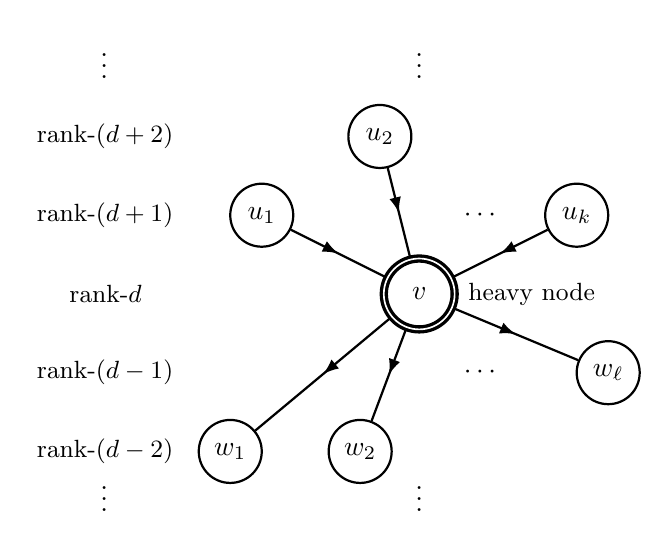
\begin{tikzpicture}[
            node/.style={circle,draw,thick,minimum size=8mm,inner sep=0pt},
            heavy/.style={circle,draw,very thick,double,minimum size=9mm,inner sep=0pt},
                        arc/.style={
                thick,
                postaction={
                    decorate,
                    decoration={
                        markings,
                        mark=at position 0.5 with {\arrow{Latex[length=2mm]}}
                    }
                }
            },
            layerlabel/.style={font=\small}
        ]
            % Depth labels
            \node at (-4,2) {$\vdots$};
            \node[layerlabel,anchor=east] at (-3.0,1) {rank-$(d+2)$};
            \node[layerlabel,anchor=east] at (-3.0,0) {rank-$(d+1)$};
            \node[layerlabel,anchor=east] at (-3.4,-1) {rank-$d$};
            \node[layerlabel,anchor=east] at (-3.0,-2) {rank-$(d-1)$};
            \node[layerlabel,anchor=east] at (-3.0,-3) {rank-$(d-2)$};
            \node at (-4,-3.5) {$\vdots$};

            % Upper layer
            \node[node] (u1) at (-2,0) {$u_1$};
            \node[node] (u2) at (-0.5,1) {$u_2$};
            \node at (0.8,0) {$\cdots$};
            \node[node] (uk) at (2,0) {$u_k$};

            % Heavy node
            \node[heavy] (v) at (0,-1) {$v$};
            \node[font=\small,anchor=west] at (0.5,-1) {heavy node};

            % Lower layer
            \node[node] (w1) at (-2.4,-3) {$w_1$};
            \node[node] (w2) at (-0.75,-3) {$w_2$};
            \node at (0.8,-2) {$\cdots$};
            \node[node] (wk) at (2.4,-2) {$w_\ell$};

            % Indication that the DAG continues
            \node at (0,2) {$\vdots$};
            \node at (0,-3.5) {$\vdots$};

            % Arcs through v
            \draw[arc] (u1) -- (v);
            \draw[arc] (u2) -- (v);
            \draw[arc] (uk) -- (v);

            \draw[arc] (v) -- (w1);
            \draw[arc] (v) -- (w2);
            \draw[arc] (v) -- (wk);
        \end{tikzpicture}
        \caption{Original derivation DAG with a heavy node \(v\).}
        \label{fig:heavy-node-before}
    \end{subfigure}
    \hfill
    \begin{subfigure}[b]{0.45\textwidth}
        \centering
        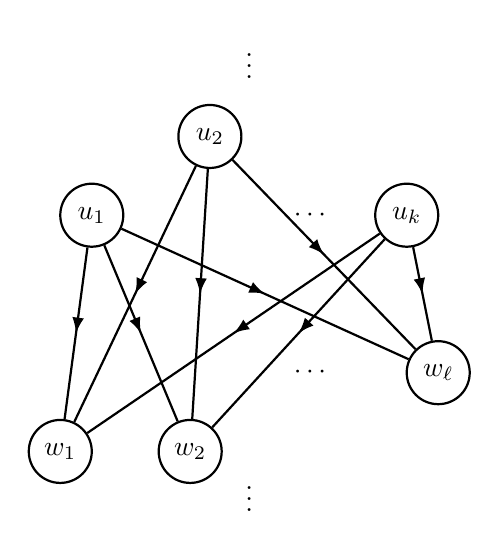
\begin{tikzpicture}[
            node/.style={circle,draw,thick,minimum size=8mm,inner sep=0pt},
            arc/.style={
                thick,
                postaction={
                    decorate,
                    decoration={
                        markings,
                        mark=at position 0.5 with {\arrow{Latex[length=2mm]}}
                    }
                }
            },
            layerlabel/.style={font=\small}
        ]

            % Upper layer
            \node[node] (U1) at (-2,0) {$u_1$};
            \node[node] (U2) at (-0.5,1) {$u_2$};
            \node at (0.8,0) {$\cdots$};
            \node[node] (Uk) at (2,0) {$u_k$};

            % Lower layer
            \node[node] (W1) at (-2.4,-3) {$w_1$};
            \node[node] (W2) at (-0.75,-3) {$w_2$};
            \node at (0.8,-2) {$\cdots$};
            \node[node] (Wk) at (2.4,-2) {$w_\ell$};

            % Indication that the DAG continues
            \node at (0,2) {$\vdots$};
            \node at (0,-3.5) {$\vdots$};

            % Replacement arcs
            \foreach \U in {U1,U2,Uk} {
                \foreach \W in {W1,W2,Wk} {
                    \draw[arc] (\U) -- (\W);
                }
            }
        \end{tikzpicture}
        \caption{New derivation DAG after eliminating $v$.}
        \label{fig:heavy-node-after}
    \end{subfigure}
    \caption{Elimination of a heavy node.}
    \label{fig:heavy-node-removal}
\end{figure}
Denote by $(\tilde{D}=(\tilde{V}, \tilde{E}),\tilde{d},\tilde{\lambda})$ the derivation DAG after elimination of heavy nodes. Each arc $a \in \tilde{E}$ corresponds to a path $\pi(a)$ of $D$, whose arcs are those which were combined in the first step of the elimination process, in order to form this new arc $a$. For arcs that existed in $D$ already, the path corresponds to the original arc. Notice that
%
\begin{equation}
\label{eq:loss_on_arc}
\tilde{\lambda}(a) \ge (1-\eps)^{\ell(a) - 1} \lambda(\pi(a))
\end{equation}
%
for all $a \in \tilde{E}$, where $\ell(a)$ denotes the length of $\pi(a)$. For $v \in \tilde{V}$, we denote by $\tilde{c}_v x \le \tilde{\rhs}_v$, and $\tilde{c}^*_v \le \tilde{\rhs}_v$ the Gomory cut and fractional inequality derived by $(D,d,\lambda)$ corresponding to node $v$. %Moreover, let $\tilde{c}^* := \tilde{c}_s$.

\begin{lemma} \label{lem:loss_control}
For all nodes $v \in \tilde{V}$ with $d(v) \le 1$, we have $\tilde{c}^*_v = c^*_v$ and for all nodes $v \in \tilde{V}$ with $d(v) > 1$, we have $\tilde{c}^*_v \ge (1-\eps)^{d(v)-1}c^*_v$. Moreover, we have $\tilde{\rhs}_v = \rhs_v$ for all nodes $v \in \tilde{V}$. 
\end{lemma}

\begin{proof}
The statement concerning nodes $v \in \tilde{V}$ with $d(v) \le 1$ is straightforward since no descendant of $v$ in $D$ got eliminated. Now let $v \in \tilde{V}$ have $d(v) > 1$. For every path $\tilde{\pi}$ in $\tilde{D}$, we have a corresponding path $\pi$ in $D$ obtained by concatenating the paths $\pi(a)$ for all arcs $a$ in $\tilde{\pi}$. By \eqref{eq:loss_on_arc}, we have $\tilde{\lambda}(\tilde{\pi}) \ge (1-\eps)^{d(v)-1} \lambda(\pi)$. The first part of the lemma follows from Lemma~\ref{lem:decomposition_into_paths}.

In order to establish the second part, it suffices to consider the case where a single heavy node $v_0 \in V$ gets eliminated. Let $u \in N^-(v_0)$. When we compare the expressions for $\rhs_u$ and $\tilde{\rhs}_u$, we see that the only difference is that the term $\lambda(u,v_0) \rhs_{v_0}$ in $\rhs_u$ gets replaced with $\sum_{w \in N^{+}(v_0)} \tilde{\lambda}(u,w) \rhs_w$ in $\tilde{\rhs}_u$ (all out-neighborhoods are computed in $D$). Now,
$$
\sum_{w \in N^{+}(v_0)} \tilde{\lambda}(u,w) \rhs_w
= 
\sum_{w \in N^{+}(v_0)}  
\frac{\rhs_{v_0}}{\sum_{w \in N^{+}(v_0)} \lambda(v_0,w) \rhs_w}
\lambda(u,v_0) \lambda(v_0,w) \rhs_w
=
\lambda(u,v_0) \rhs_{v_0}\,.
$$
Hence, $\rhs_u = \tilde{\rhs}_u$ for all predecessors of $v_0$, which implies $\rhs_v = \tilde{\rhs}_v$ for all $v \in \tilde{V}$.
\end{proof}

\subsection{Construction of the row distribution from the derivation DAG}

With the machinery introduced in Section \ref{subsec:derivation-DAG}, we are now ready to prove Lemma \ref{lem:distribution}.

    Let $c^\intercal x \le \rhs$ be a Gomory cut of rank-$t$ for $P$, with $c \in \Z^n_{\ge 0}$ and $\rhs \in \Z_{\ge 1}$. Assume that $\rhs < 1/\eps$. Following Section \ref{subsec:derivation-DAG}, we construct the derivation DAG of $c^\intercal x \le \rhs$ and eliminate the heavy nodes to get the modified derivation DAG $\tilde{D}=(\tilde{V}, \tilde{E})$, which will be used throughout the proof.
    
    Consider the following process for sampling a row index $i \in [m]$. We start at the source node $s \in \tilde{V}$ and we move from node to node following the arcs of $\tilde{D}$. 
    % Sitting at $u \in \tilde{V}$, we move to out-neighbor $v \in N_{\tilde{D}}^+(u)$ with probability proportional to $\tilde{\lambda}(u,v)$. 
    For each $u \in \tilde{V}$ and one of its out-neighbor $v \in N_{\tilde{D}}^+(u)$, define
    $$
    p(u,v) := \frac{\tilde{\lambda}(u,v)}{\sum_{w \in N_{\tilde{D}}^+(u)} \tilde{\lambda}(u,w)}
    $$
    which is the probability to follow the arc $(u,v)\in \tilde{E}$ when based at $u$. 
    For all $v \in \tilde{V}$ we have $1 \le \tilde{\rhs}_v \le 1/\eps$, thus for all $v \in \tilde{V}$ with $d(v) > 0$ we have
    $$
    \sum_{w \in N_{\tilde{D}}^+(v)} \tilde{\lambda}(v,w) \le \left\lceil\frac{1}{\eps}\right\rceil \le \frac{1+\eps}{\eps}.
    $$ 
	For every $i \in [m]$ and every directed path $\pi \in \mathcal{P}(s,i)$ we set $p(\pi):= \prod_{(u,v)\in \pi}p(u,v)$. Then, 
    \begin{equation*}
        p(\pi) \ge \left(\frac{\eps}{1+\eps}\right)^{\numrounds} \tilde{\lambda}(\pi).
    \end{equation*} 
    Finally, define 
    \begin{equation}\label{eq:sampling-prob-rank-t}
        p(i) := \sum_{\pi \in \mathcal{P}_{\tilde{D}}(s,i)} p(\pi),
    \end{equation}
    which is the probability that a row $i \in [m]$ is sampled. For each fixed $j \in [n]$, we have
    %
    \begin{align*}
	    \proba_{i \sim_p [m]} [j \in N(i)] &=
    \sum_{i \in [m]} A_{ij} p(i) \\
	    &=\sum_{i \in [m]} \sum_{\pi \in \mathcal{P}_{\tilde{D}}(s,i)} A_{ij} p(\pi)\\
    &\ge \sum_{i \in [m]} \sum_{\pi \in \mathcal{P}_{\tilde{D}}(s,i)} A_{ij} \left(\frac{\eps}{1+\eps}\right)^{\numrounds} \tilde{\lambda}(\pi)\\
    % &= \left(\frac{\eps}{1+\eps}\right)^{\numrounds} \tilde{c}^*_j\\
    &\ge \left(\frac{\eps}{1+\eps}\right)^{\numrounds} (1-\eps)^{\numrounds-1} c^*_j\\
    &\ge \eps^\numrounds (1-\eps)^{2\numrounds-1} c_j\,.
    \end{align*}
    Therefore for the coverage probability of $j\in \supp(c)$, we have
    \begin{align*}
    \sum_{i: j \in N(i)} p(i) &\ge \sum_{i: j \in N(i)} A_{ij} p(i) \\
    &= \sum_{i \in [m]} A_{ij} p(i) - \sum_{i \in [m] \atop A_{ij} < \threshold} A_{ij} p(i)\\
    &\ge \eps^\numrounds (1-\eps)^{2\numrounds-1} c_j - \sum_{i \in [m]} p(i) \cdot \tau \\
    &\ge \eps^\numrounds (1-\eps)^{2\numrounds-1} - \tau \,. \qedhere
    \end{align*}
    % In this case, the lower bound on the coverage probability $\gamma$ equals the threshold. {\color{red} We could have used a single parameter!}


\subsection{Proof of Theorem~\ref{thm:main-1}}

We restate Theorem~\ref{thm:main-1} here for convenience.
\approxcg*
\begin{proof}
    % Here is how we set the parameters, for given $\eps > 0$ and $\numrounds$:
    % %
    % \begin{align*}
    % \covproba = \threshold &= \frac{1}{2} \left(\frac{\eps}{1+\eps}\right)^{\numrounds} (1-\eps)^{\numrounds-1}\\
    % \numrows &= \ceil{1/\covproba \cdot \ln (1+1/\eps)}\\
    % &\le \frac{1}{\eps^{\numrounds+2}}\\
    % \end{align*}
    
    % For a feasible $x \in \{0,1\}^n$, and $I \subseteq [m]$ with $|I| \le r$, we have the following bound:
    % %
    % \begin{align*}
    % \sum_{j \in N(I)} x_j
    % &\le r \cdot \frac{1}{\tau}\\
    % &\le \frac{1}{\eps^{2\numrounds+3}}
    % \end{align*}
    
    % The final size bound we get for the extended formulation is
    % $$
    % m^{(1/\eps)^{\numrounds+O(1)}} n^{(1/\eps)^{2\numrounds+O(1)}}
    % $$
	We can assume without loss of generality that $A\in [0,1]^{m\times n}$. Every variable
	with a coefficient greater than $1$ in some row cannot be $1$ and can therefore be removed.
    Construct the relaxation $Q \subseteq \R^n_{\geq 0}$ of the integer hull of $P$ as in Lemma \ref{lem:construction-r-neighborhood-exact-relaxation} with the parameters
    \begin{equation*}
	    \gamma = \threshold = \frac{1}{2} \eps^{\numrounds} (1-\eps)^{2\numrounds-1} \quad \text{ and }
    \quad \numrows = \ceil{1/\covproba \cdot \ln (1+1/\eps)} \,.
    \end{equation*}
	The relaxation $Q$ is $r$-neighborhood-exact and is of size
	\begin{equation*}
		O(m^r n^{1 + r/\tau}) \le (mn)^{(1/\eps)^{O(t)}} \, .
	\end{equation*}
    %which gives the desired size of $Q$: Indeed, using $1+\eps \le (1-\eps)^{-1}$ and $\eps/(1-\eps) \le 2$, we have
    %$$
    %1/\gamma \le 2 \left(1/\eps\right)^{\numrounds} 
    %\left(\frac{1}{1-\eps}\right)^{2\numrounds}
    %%= 2 \left(1/\eps\right)^{\numrounds} 
    %%\left(1+\frac{\eps}{1-\eps}\right)^{2\numrounds}
    %\le 2 \left(1/\eps\right)^{\numrounds} 
    %\mathrm{e}^{\frac{2 \numrounds \eps}{1-\eps}}
    %\le 2 \left(1/\eps\right)^{\numrounds} 
    %\mathrm{e}^{4\numrounds}\,.
    %$$    
	We will now show that $Q$ gives a $(1+\eps)^\numrounds$-approximation of $P^{(\numrounds)}$ by induction on $t$. The base case $t=0$ holds because of $P^{(0)} = P$. For the induction step, assume that $Q\subseteq (1+\eps)^{t-1}P^{(t-1)}$, and consider an inequality $c^\intercal x \le \floor{\delta}$ that is valid for $P^{(\numrounds)}$ with $c \in \Z^n_{\ge 0}$ and $\floor{\delta} < 1/\eps$.
	By Lemma~\ref{lem:distribution} there is a distribution $p\in \Delta_{m-1}$ with
	\begin{equation*}
		\proba_{i \sim_p [m]} [j \in N(i)] \ge \eps^{\numrounds} (1-\eps)^{2\numrounds-1} - \tau = \gamma \,.
	\end{equation*}
	Thus, by Lemma~\ref{lem:averaging} it follows that $c^\intercal x \le (1+\eps)^\numrounds \floor{\delta}$ is valid for $Q$. From Lemma~\ref{lem:induction} it follows that $Q\subseteq (1 + \eps)^t P^{(t)}$.
\end{proof}

% Section on improved depth upper bound for hypergraph matching 
%\section{Improved depth bound of local constraints for
  \section{Hypergraph matching}\label{sec:hypergraph-matching}
Given a hypergraph $G = (V, E)$, the maximum matching problem on $G$ is to find a maximum cardinality subset $E^\prime \subseteq E$ of hyperedges so that each vertex $v\in V$ is incident to at most one hyperedge $e \in E^\prime$. 
For the unweighted maximum matching problem in hypergraph, we have the following standard LP relaxation:
    \begin{align*}
      \max & \quad \sum_{e\in E} x_e \\
      \text{s.t.}
      & \quad \sum_{e\in\delta(v)} x_e \leq 1, \forall \, v\in V,\\
      & \quad x_e \geq 0, \forall \, e\in E.
    \end{align*}
A hypergraph $G = (V, E)$ is called $k$-uniform if $|e|=k$ for each $e \in E$. In this section, we study the (unweighted) maximum matching problem for $k$-uniform hypergraphs and show the following.
%In \cite{st10}, it is shown that $O(k^2)$ rounds of Gomory-closure operation is enough to reduce the integrality gap of the LP to $(k+1)/2$. 
%Motivated by Section~\ref{sec:r-neighbor}, we improve their result by showing that $O(\log k)$ rounds of Gomory-closure operation suffices to achieve the same integrality gap.
% \begin{proposition}
%     For the maximum matching problem in $k$-uniform hypergraphs $H=(V,E)$, it suffices to apply $O(\log k)$ rounds of CG to the standard LP relaxation $P$ to reduce the integrality gap to $(k+1)/2$.
% \end{proposition}

\hyper*

\begin{proof}
    It was shown in \cite{cl12}, that the following LP has integrality gap of at most $(k+1)/2$:
    \begin{align*}
      \max & \quad \sum_{e\in E} x_e \\
      \text{s.t.}
      & \quad \sum_{e\in\delta(v)} x_e \leq 1, \forall \, v\in V, \\
      & \quad \sum_{e\in K} x_e \leq 1, \forall\;\text{intersecting family}\; K\subseteq E, \\
      & \quad x_e \geq 0, \forall \, e\in E.
    \end{align*}
    Let $K \subseteq E$ be an intersecting family, that is, a family of hyperedges with pairwise intersection.
    We claim that the rank of the clique inequality $x(K):=\sum_{e\in K} x_e\leq 1$ is $2+2\log r$, provided that $K$ has a hitting set of size $r$.
	By relabelling, assume that the vertices $\{1,2,\dotsc,r\} \subseteq V$ form a hitting set of $K$. Let $K_i$, $i\in\{1,2,\dotsc,r\}$, denote the edges in $K$ that contain vertex $i$.
	Then $K_1\cup \cdots\cup K_r = K$. Note that $x(K_i)\leq 1$ is valid for $P$ for each $i = 1,\dots, r$. Set $k_i := |K_i|$.
    Consider $K_1$ and $K_2$ (assume that both are non-empty). Since $K$ is a clique, we have that $x_i + x_j\leq 1$ is valid for $P$, for each $i \in K_1, j \in K_2$. 
    Hence for any fixed $i \in K_1$, we have that 
    \[x_i + \frac{1}{k_2} x(K_2) \leq 1\] 
    is valid for $P$. Also, 
    \[\frac{k_2-1}{k_2} x(K_2) \leq \frac{k_2-1}{k_2}\] 
    is valid for $P$. Hence by adding both inequalities we get that 
    \[x_i + x(K_2) \leq 1 + \frac{k_2-1}{k_2}\] 
    is valid for $P$. Thus, $x_i + x(K_2) \leq 1$ is valid for the first closure $P^\prime$ for every $i \in K_1$. 
    Similarly, $x(K_1) + x_j \leq 1$ is valid for $P^\prime$, for every $j \in K_2$. 
    Now we can average these inequalities to see that 
    \begin{equation*}
        \frac{1}{k_1} x(K_1) + x(K_2) \leq 1\quad \text{and} \quad x(K_1) + \frac{1}{k_2} x(K_2) \leq 1
    \end{equation*} 
    are valid for $P^\prime$. Without loss of generality, we may assume that $k_1\leq k_2$, hence by summing the two inequalities above and scaling by $k_2/(k_2+1)$ we have
    \[
	    \frac{k_1+1}{k_1}\cdot \frac{k_2}{k_2+1} x(K_1) + x(K_2) \le \frac{k_2}{k_2+1} x(K_1) + \left(\frac{1}{k_1} x(K_1) + x(K_2)\right) \leq \frac{k_2}{k_2+1} + 1 < 2 \, ,
    \]
    which implies that $x(K_1) + x(K_2) \leq 1$ is valid for the second closure $P^{\prime\prime}$.
    This means that after two rounds of Gomory-closure operation, we can ``merge'' every two consecutive cliques in $K_1, \cdots, K_r$ into a single clique. 
    By repeatedly merging, we get a bound of $2 \ceil{\log r} \leq 2+2\log r$ on the rank of $x(K) \leq 1$.

    By taking the $k$ vertices of one hyperedge in $K$ we can see that $K$ always has a hitting set of size $k$.
	Thus, we can take $r=k$. The claim above implies that $x(K)\leq 1$ can be captured in $O(\log k)$ rounds of Gomory-closure operation. This completes the proof.
      \end{proof}


%%% Local Variables:
%%% mode: LaTeX
%%% TeX-master: "../main"
%%% End:


% Section on the second main result
\section{Extended formulation from communication complexity}
\label{sec:depth-independent}
%\lars{Changes:
%\begin{itemize}
%	\item Remove remark about approximative version of Lemma \ref{lem:small-rhs}. We cannot really gain much from approximating, because setting $\epsilon < 1/\delta_{\max}$ recovers the exact variant. 
%	\item required that incidence vector of tight set $S$ is in $P$. Otherwise it is forcing set is everything.
%	\item removed the upper bound that Alice maintains, since it is not really used in the writing.
%	\item I removed the base case $n = 1$. It does not seem necessary to me to handle this seperately.
%	\item Spelled out the case where Bob sends $S$
%\end{itemize}
%}
Towards Theorem~\ref{thm:main-2}, the main technical challenge is to prove the following lemma about capturing all valid inequalities for the integer hull with small right-hand sides. 

\begin{lemma} \label{lem:small-rhs}
Let $P = \{x \in \R^n_{\ge 0} : Ax \le b\}$ be a polytope contained in $[0,1]^n$, where $A \in \R_{\ge 0}^{m \times n}$ and $b \in \R_{\ge 0}^m$. Let $\rhs_{\max} \in \Z_{\ge 1}$. There exists a polyhedral relaxation $R$ of the integer hull of $P$ such that $R$ has a size-$n^{2
\rhs_{\max} \log n}$ extended formulation and every inequality $c^\intercal x \le \rhs$ with integer coefficients and $\rhs \le \rhs_{\max}$ that is valid for the integer hull of $P$ is also valid for $R$.
\end{lemma}
%We note that for the proof of Theorem~\ref{thm:main-2} it would suffice that $R$ gives an $(1+\eps)$-approximation for the valid inequalities of the integer hull of $P$ with right-hand side at most $\rhs_{\max}$, but we could not exploit this to decrease the extension complexity of $R$.

\begin{proof}
We provide a deterministic communication protocol with complexity $O(\rhs_{\max} \log^2 n)$ which solves the following communication problem:
There are two players Alice and Bob. Alice is given an inequality $c^\intercal x \le \rhs$ that is valid for the integer hull of $P$, where $c \in \Z^n_{\ge 0}$, $\rhs \in \{1,\ldots,\rhs_{\max}\}$. We write $K:=\supp(c)$. Bob is given a feasible integer solution $z \in P \cap \Z^n = P \cap \{0,1\}^n$. We write $B:=\supp(z)$. Their task is to compute the \emph{slack} $\rhs - c^\intercal z \in \{0,\ldots,\rhs\}$ by exchanging as few bits as possible. In this context, they do so deterministically. The number of bits exchanged in the worst case is the \emph{complexity} of the protocol. Each player knows $P$ and their own input, but does not know the input of the other player. The players are otherwise not assume to be computationally bounded.

By known results in~\cite{yan88}, which connect communication protocols and extended formulations, our protocol gives an extended formulation for $Q$ of size $2^{O(\rhs_{\max} \log^2 n)} = n^{O(\rhs_{\max} \log n)}$. In fact, our protocol generalizes Yannakakis' protocol~\cite{yan88} for the clique versus stable set problem, to any packing problem and any right-hand side.

For any set $S \subseteq [n]$ with $|S| \le \rhs$, we define the $\forcingset(S)$ to be the set of all indices $j' \in [n]$ such that $x_{j’} = 0$ in each feasible integer solution $x$ such that $x_j = 1$ for all $j \in S$. 
Define $\forcing(S)$ to be the size of its forcing set. We call a set $S \subseteq K$ \emph{tight} if $\sum_{j \in S} c_j = \rhs$ and $\mathbf 1_S \in P$. Notice that tight sets have at most $\rhs$ elements, since $c_j \ge 1$ for all $j\in K$.

In the protocol, Alice and Bob try to apply a number of simplifying rules in the given order until one of them succeeds. Then
they start again at the first rule.
In this process, they may identify elements $j\in K\cap B$, which they then contract (set to $1$).
This means they both remove it from the instance, Alice reduces $\rhs$ by $c_j$ and they compute the slack in
the remainder instance, which they then output for the overall instance as well.
%Alice keeps in her memory an upper bound $\sigma$ for the slack, which is initially $\rhs$ and is decreased by $c_j$ whenever the players find any element $j \in K \cap B$. When the protocol stops, Alice outputs $\sigma$. In order to guarantee that the output of the protocol is correct, it suffices to make sure that all elements in $K \cap B$ are discovered in the process, and known to Alice.

\paragraph{Rule 1.} If $n = 0$ or $\rhs = 0$ then the protocol stops and Alice outputs $\rhs$. 
	%If $n = 1$, then Bob simply sends one bit to Alice to tell her what $B$ is, which can either be the empty set or the set containing the single element in the instance. Alice can then compute and output the slack.

\paragraph{Rule 2.} Bob looks for a set $S \subseteq B$ of size at most $\rhs$ with $\forcing(S) \ge n/2$. 
If he finds such a set, he informs Alice of this and sends all elements in $S$ one after the other.
After each element $j$, Alice tells Bob whether $j\in K$.
Then, they both contract (set to $1$) the variables $x_j$ for $j \in K \cap S$ and delete (set to $0$) the variables $x_j$ for $j \in \forcingset(S)$, and recurse on a smaller problem with at most $n/2$ variables and right-hand side at most $\rhs$. This is safe since $\forcingset(S) \cap K = \emptyset$. 
If Bob fails to find such a set $S \subseteq K$ with $\forcing(S) \ge n/2$, he informs Alice and the protocol continues to the next rule.

\paragraph{Rule 3.} Alice looks for a tight set $S \subseteq K$ with $\forcing(S) < n/2$. Recall that such a set satisfies $1 \le |S| \le \rhs$. If she can find such a set, we proceed similar to before: she sends to Bob all the elements $j\in S$ and Bob tells Alice whether $j \in B \cap S$ or not. Afterwards, both contract the variables $x_j$ for $j \in B \cap S$ and delete the variables $x_j$ for $j \notin \forcingset(S)$, and recurse on a smaller problem with at most $n/2$ variables and right-hand side at most $\rhs$. This is again safe since $K \subseteq \forcingset(S)$. If Alice fails to find a tight set $S \subseteq B$ with $\forcing(S) < n/2$, she informs Bob of this and they continue the protocol.

Suppose that Rules 1-3 have been applied until exhaustion. Then the following properties hold:
%
\begin{enumerate}[(P1)]
\item every $S \subseteq B$ with $|S| \le \rhs$ has $\forcing(S) < n/2$;
\item every tight set $S \subseteq K$ has $\forcing(S) \ge n/2$.
\end{enumerate}

\paragraph{Rule 4.} If none of the players is able to find a set $S$ contained in their respective set which allows them to make progress, they add to the inequalities defining $P$ all the inequalities of the form $\sum_{j \in S} x_j \le |S| - 1$ where $S \subseteq [n]$ has size at most $\rhs$ and $\forcing(S) \ge n/2$. They can do so without communicating. Let $\tilde{P} \subseteq P$ denote the resulting polytope. By (P1), $z$ is an integer point of $\tilde{P}$. By (P2), $c^\intercal x \le \rhs - 1$ is valid for the integer hull of $\tilde{P}$: indeed, otherwise there would exist an integer solution $y \in \tilde{P} \cap \{0,1\}^n$ with $c^\intercal y > \rhs - 1$. Since $\tilde{P} \subseteq P$, we have $y \in P \cap \{0,1\}^n$, implying that $c^\intercal y \le \rhs$ and therefore $c^\intercal y = \rhs$. Let $S := K \cap \supp(y)$. By (P2), we have $\forcing(S) \ge n/2$. Hence the constraint $\sum_{j \in S} x_j \le |S| - 1$ is one of the constraints defining $\tilde{P}$, however it is violated by $y$ since $y_j = 1$ for all $j \in S$, this contradicts our assumption that $y \in \tilde{P}$. The players can recurse on $\tilde{P}$ with inputs $c^\intercal x \le \rhs - 1$ (for Alice) and $z$ (for Bob). To the computed slack, they then add $1$ and output it.

Let $f(n,\rhs)$ denote the number of bits exchanged by the protocol above. Then $f(n,\rhs) = 0$ when $n = 0$ or $\rhs = 0$, and $f(1,\rhs) = 1$. Otherwise, we have
%
\begin{align*}
f(n,\rhs) \le \max \{ &1 + \rhs (\ceil{\log n}+1) + f(\floor{n/2},\rhs),\\ 
       &1 + 1 + f(n,\rhs-1)\}.
\end{align*} 
%	\lars{I do not feel confident about the exact constants in the recurrence. Perhaps it would be better to use $O(\cdot)$?}
%
We infer from this that $f(n,\rhs) \le 2 \rhs \log^2 n$ for $n \ge 2$ and $\rhs \ge 1$.
\end{proof}

We are now ready to prove Theorem~\ref{thm:main-2}, which we restate here for the convenience.

\ef*

\begin{proof}
	Let $Q := P \cap R$, where $R$ is the relaxation from Lemma~\ref{lem:small-rhs} with $\delta_{\max} = \lfloor 1/\eps \rfloor$. We prove $Q \subseteq (1+\eps)^{\numrounds} P^{(
\numrounds)}$, by induction on $t \in \Z_{\ge 0}$. 

For $t = 0$, we have $Q \subseteq P = (1+\eps)^0 P^{(0)}$.

Now assume that $\numrounds \ge 1$, and invoke Lemma~\ref{lem:induction}. By induction, we know that $Q \subseteq (1+\eps)^{\numrounds-1} P^{(
\numrounds-1)}$. Hence, Condition~(i) of Lemma~\ref{lem:induction} is satisfied. Moreover, $Q \subseteq R$. By Lemma~\ref{lem:small-rhs}, this in particular implies that Condition~(ii) of Lemma~\ref{lem:induction} is satisfied. We conclude that $Q \subseteq (1+\eps)^{\numrounds} P^{(\numrounds)}$.
\end{proof}

% {\color{red} TODO: discuss that this shows the existence of $Q$, but we do not know if $Q$ can be constructed in polynomial-time. Have to be careful here.}
\begin{remark}
	Note that Theorem~\ref{thm:main-2} shows the existence of such a relaxation $Q$, but it is not known if $Q$ can be constructed in polynomial-time. 
\end{remark}




% AI statement
\section*{AI statements}
AI was not used as a tool for writing this article, nor as a tool to find proofs of any parts of the theorems of this paper. 
AI was used for literature research and generating the tikz code of the figure. This exposition, theorems, and proofs are solely from the authors. 

\phantomsection
\addcontentsline{toc}{section}{References}
\printbibliography

\appendix

\section{Approximation factor of Theorem~\ref{thm:main-1}}\label{appendix:approx-factor}
In Theorem~\ref{thm:main-1}, $(1+\eps)^\numrounds$ is the target approximation factor. By taking $\eps = (1+\tilde{\eps})^{1/\numrounds} - 1$, or equivalently $\tilde{\eps} = (1+\eps)^t-1$, one can translate the result as a $(1+\tilde{\eps})$-approximation of the $\numrounds$-th Gomory closure. 
By the Newton's binomial theorem, we have
\begin{align*}
    \tilde{\eps} = (1+\eps)^t - 1 = \sum_{k=0}^\numrounds {\numrounds \choose k} \eps^k - 1 = \rb{1+t\eps+\binom{t}{2}\eps^2 +\cdots} - 1 = t\eps + O(\eps^2).
\end{align*}
After ignoring the higher order terms, we get $\tilde{\eps} \approx t\eps$.

\section{Inductive lemma for covering problems}\label{appendix:covering}
% \larstodo{do we refer to this anywhere in the main body?}
The following lemma is a natural analog of Lemma~\ref{lem:induction} to covering polytopes.
\begin{lemma} \label{lem:induction-covering}
    Let $\numrounds \in \Z_{\ge 1}$ and let $Q \subseteq \R^n_{\ge 0}$ be any convex relaxation of blocking type for the integer hull of $P$ such that 
    %
    \begin{enumerate}[(i)]
    \item $(1+\eps)^{\numrounds-1}Q \subseteq P^{(\numrounds-1)}$,
    \item for every inequality $c^\intercal x \ge \ceil{\delta}$ that is valid for $P^{(\numrounds)}$ with $c \in \Z^n_{\ge 0}$ and $\ceil{\delta} < (1+\eps)/\eps$, the inequality $c^\intercal x \ge (1+\eps)^\numrounds \ceil{\delta}$ is valid for $Q$. 
    \end{enumerate}
    %
    Then $(1+\eps)^{\numrounds}Q \subseteq P^{(\numrounds)}$.
\end{lemma}
\begin{proof}
    Consider any valid inequality $c^\intercal x \ge \ceil{\delta}$ for $P^{(\numrounds)}$ where $c \in \Z^n_{\ge 0}$, $\delta \ge 1$ and $c^\intercal x \ge \delta$ is valid for $P^{(\numrounds-1)}$. Our goal is to show that $c^\intercal x \ge (1+\eps)^{-\numrounds} \floor{\delta}$ is valid for $Q$. 
    %
        If $\ceil{\delta} < (1+\eps)/\eps$, this holds by (ii). Hence, we may assume that $\ceil{\delta} \ge (1+\eps)/\eps$. Since $c^\intercal x \ge \delta$ is valid for $P^{(\numrounds-1)}$ and $(1+\eps)^{\numrounds-1} Q \subseteq P^{(\numrounds-1)}$, the inequality $c^\intercal x \ge (1+\eps)^{1-\numrounds} \delta$ is valid for $Q$. 
    %
    Using that $\delta \ge \ceil{\delta} - 1 \ge (1+\eps)^{-1} \ceil{\delta}$, we conclude that $c^\intercal x \ge (1+\eps)^{-\numrounds} \ceil{\delta}$ is valid for $Q$.
\end{proof}
As commented earlier, Lemma~\ref{lem:induction-covering} together with the results from \cite{fhw21} give an extended formulations of polynomial size which approximates the covering polytope within $(1+\eps)$.


\end{document}

%%% Local Variables:
%%% mode: LaTeX
%%% TeX-master: t
%%% reftex-default-bibliography: ("papers.bib" "mybib.bib" "books.bib" "refs.bib")
%%% End:
